% press command+option+B to build, or change "Auto Build: Run" in Settings.

\documentclass{book}

\usepackage{xeCJK}
\usepackage{geometry}
\usepackage{titlesec}

\usepackage{underlin}
\usepackage{wrapfig}
\usepackage{caption}
\usepackage{graphicx}
\usepackage{psfrag}
\usepackage{subfig}
% \usepackage{dvips}
\usepackage{pdfpages}
\usepackage{multirow}%表格合并行列单元格

% 分栏并浮动图片
\usepackage{float}
\usepackage{multicol}
\usepackage[none]{hyphenat}
\usepackage{appendix}

% 数学
\usepackage{unicode-math}%正体希腊字母
\usepackage{mathrsfs}
\usepackage{amsfonts}
\usepackage{bm}
\usepackage{bbm}
% \usepackage{amsmath}
% \usepackage{amssymb}

% 设置图书版式
\usepackage{marginnote}%侧栏
\usepackage{fancyhdr}%页眉页脚页码
\usepackage{indentfirst}%首段空两格
\usepackage{mdframed}%加阴影
\usepackage{xcolor}%特殊字体颜色

\usepackage{setspace}%行距

\usepackage{hyperref}%所有网页用超链接同步挂靠
\usepackage{xpatch}%设置verbatim前后间距

\usepackage{mflogo}%METAPOST和METAFONT logo

%行号
\usepackage{lineno}

%圆角边框
\usepackage{fancybox}

%首字下沉
\usepackage{lettrine}

%原书使用的特殊符号输入
\usepackage{pifont}

%特殊字体
\usepackage{fontspec}

\def\codereplace#1{%代码中的<可替换>部分
    \xeCJKsetup{CJKecglue={\hskip 0pt}}
    \textsl{⟨#1⟩}}

\def\wz#1{%网址
    {\ttfamily #1}}

\def\jz#1{%原书脚注
    \footnote{#1}
}

\def\yz#1{%译注
    \footnote{\textsl{译注:}#1}
}

\def\dm#1{%代码
    \texttt{#1}}

\def\dmh#1{%代码行
    {\xeCJKsetup{CJKecglue={\hskip 0pt}}
    \char"258E \texttt{#1}}
}

%侧栏TODO三角形方向
\def\celan#1{
$\blacktriangleright$
\marginpar{
        $\blacktriangleleft$\textsf{#1}
    }
}

%bibtex logo
\def\bib{\textsc{Bib}\TeX }

%原书的圆圈感叹号
\definecolor{LightPink}{RGB}{230,173,173}
\newenvironment{exclamation}[1][!]%
{
    \begin{mdframed}[backgroundcolor=LightPink,hidealllines=true]
        {\textcircled{\scriptsize #1}} \quad
        \sffamily
}{      
    \rmfamily
    \end{mdframed}
}

%原书的圆圈i
\definecolor{LightBlue}{RGB}{173,216,230}
\newenvironment{ii}[1][i]
{
    \begin{mdframed}[backgroundcolor=LightBlue,hidealllines=true]
        {\textcircled{\scriptsize #1}} \quad
        \sffamily
}{      
    \rmfamily
    \end{mdframed}
}

\newenvironment{dmd}{%代码段
    \xeCJKsetup{CJKecglue={\hskip 0pt}}
    \vspace{0.5em}
    \ttfamily
    \setlength{\parindent}{0pt}
}{
    \rmfamily
    \vspace{0.5em}
}

%代码清单
\newenvironment{codelist}[2][TODO代码清单序号]{
    \setlength{\parindent}{0pt}
    \begin{mdframed}
        \textbf{清单 #1}
        \begin{mdframed}[backgroundcolor=lightgray,hidealllines=true]
            #2 
        \end{mdframed}
}
{
    \end{mdframed}
}

%字体
\setCJKmainfont[
    BoldFont={NotoSerifCJKsc-Bold},
    ItalicFont={Kai},
    SlantedFont={STFangsong},
    ]
    {STSongti-SC-Regular}
\setCJKsansfont[
    ItalicFont={SmileySans-Oblique},
    SlantedFont={STFangsong}]
    {NotoSansCJKsc-DemiLight}
\setCJKmonofont[
    % ItalicFont={SmileySans-Oblique},
    SlantedFont={STFangsong}]
    {STYuanti-SC-Regular}
\setmonofont[
    ItalicFont={LMMono10-Italic},
    SlantedFont={SFMono-RegularItalic}
    ]
    {LMMono10-Regular}
% \setsansfont[
%     SmallCapsFont = {NotoSansCJKsc-DemiLight}
%     ]
%     {NotoSansCJKsc-DemiLight}

%特殊字符的字体显示
\xeCJKDeclareSubCJKBlock{angleBracket}{
    "27E8 -> "27E9 %〈〉半角括号
}
\setCJKmainfont[angleBracket]{STIXTwoMath-Regular}

\xeCJKsetcharclass{"2580}{"259F}{1}%侧栏小方块示例
\xeCJKsetcharclass{"211A}{"211F}{1}%双钩R
\xeCJKsetcharclass{"0370}{"03FF}{1}%希腊字母
\xeCJKsetup{AutoFallBack=true}
\setCJKfallbackfamilyfont{\CJKrmdefault}{ArialUnicodeMS}

%带跳转的内容颜色
\definecolor{MediumBlue}{RGB}{0,0,205}
\hypersetup{
    colorlinks = true,
    linkcolor = MediumBlue
}

\title{关于\LaTeX 的那些你想知道却从不敢问的问题\\{\small 或者说,如何在不会使用\LaTeX 的情况下使用\LaTeX }\\~\\Tout ce que vous avez toujours voulu savoir sur \LaTeX \ sans jamais oser le demander\\{\small Ou comment utiliser \LaTeX \ quand on n'y connaît goutte}\\~\\ ver. 1.5}
\author{Vincent Lozano 著}

\begin{document}
\maketitle
\tableofcontents
\mainmatter

%正文版式
\newgeometry{
    % inner = 2cm, outer = 4cm,
    % top = 2.5cm, bottom=2.5cm, 
    marginparwidth = 2cm, marginparsep = 0.5cm,
    % includeheadfoot
}
\pagestyle{fancy}
\fancyhead{} 
\fancyhead[RO,LE]{\thepage}
\fancyfoot{}

%verbatim设置为不特殊打断,会根据代码内容与\verb 和\texttt混用
\setstretch{1.2}
\xpretocmd\verbatim{
    \setlength{\topsep}{0pt}
    \setlength{\partopsep}{0pt}
    }{}{\fail}

\chapter*{序}

男人的邪恶胜过女人的善良\jz{
    本书的章首引言来自《旧约》与《新约》,将它们引用在这里纯粹是我一手挑动的——有时,这些句子中带有一些与章标题相关的内容(译注:宗教相关内容按原文直译,不代表译者对任何宗教文献中任何语句的认可或否认。本书未标注“译注”字样的脚注均为原书脚注)。
}。——《便西拉智训\yz{原文如此,但作为《诗歌智慧书》一部分的《便西拉智训》(天主教译为《德勋篇》)似乎属于次经,即在一些教派中不被承认作为《圣经》的一部分出现。 
}》42:14

\section*{从前……}

一切始于1990年年初。我当时正在PC 286计算机上使用称为\textit{WordPerfect}的软件,以此入门人们所谓的“文字处理”。这款软件现在仍然存在,并且由Corel公司维护,运行在日后拥有响当当名头的MS-DOS中。MS-DOS集成了用以粗略预览文档的接口,尤其允许用户“看到代码”,也就是借助一种标记语言将文档可视化,以灵活地控制。

稍晚些时间,随着Windows 3.1迅速风靡,人们突如其来地追求图形界面,我虽然仍情有不甘,却逐渐说服了自己去使用那款在今天很出名的文字处理软件——的2.0版(后面还带个小小的字母,在当时那可真是重大的升级)……但我日后才知道,这个版本有个很有趣的“特性”:文件体积过大,超过了某个特定的值时,会出现保存失败的情况!这时,你既不能保存,也不能恢复文档。有些头铁的朋友尝试先删除几行再保存,但这种撞大运的解决方案并没能成功……

当时,大家毫不掩饰地嘲讽这些“你懂的”公司制作的软件\jz{
    这些被嘲讽的对象中,我们可以看到一些名场面:通用汽车公司老板对比尔·盖茨挑衅性言论的回应(译注:可能是指比尔·盖茨的观点,即如果汽车工业能够像计算机领域一样发展,那么一辆汽车只需要25美元就能买到,并且消耗1加仑汽油就能跑1000英里。作为回应,通用汽车方面罗列了一系列言论来嘲讽,例如“如果那样,那么想要汽车熄火,需要点击开始菜单”),以及罗伯托·迪·科斯莫(Roberto Di Cosmo)的“赛博空间中的陷阱”(piège dans le cyberespace)。
}——这里就不点名了。我周围的大多数人躺平地选择了接受,认为使用这些堂而皇之不给出警告的可悲的跟风之流是正常现象。软件的这种“特性”坚定了我的信念:\textit{我绝不使用这种软件}。当时还在攻读工程师学位的我意识到,我今后的部分工作将会集中在起草文档和使用通用的信息系统上。为此,我需要足够健壮的工具。

我是在让·莫奈大学(Université Jean Monnet)和圣-埃蒂安高等矿业学校(École des Mines de Saint-Étienne)攻读DEA(现在叫master recherche)\jz{
    译注:DEA即diplôme d'études approfondies,法国教育体系下的一种学位。
}时相继接触UNIX和Linux的。那时(1993~1994年),在我刚写论文的开头时,“拉泰克”(latèque)这个词就开始围着我转。这里问题似乎是要找到一款能排出数学公式的软件,而说到撰写理科文档,\LaTeX 似乎显然是避不开的\textit{唯一}答案。说实话,找软件这种问题甚至都根本没出现过!

于是,我着手把这个叫做\LaTeX 的“玩意儿”装在Mac系统(安装的发行版叫Oz\TeX )和另一个由古登堡(Gutenberg)协会支持的发行版系统——Solaris上。为此,我还得去收买一个系统管理员,让他同意创建一个特权用户\texttt{texadm},用来管理那个发行版……

1994年年初,我带着坚定的意志使用\LaTeX 开始写论文。在1995年,在被我发现的种种技巧激起的兴趣的巨大感召下,% 此句翻译不好:enthou- siasmé par ce que je découvrais, TODO
我着手为同事和实验室起草用于入门\LaTeX 的指导手册。这个手册就是本书的原型。在1997年,在练习了两年并一只脚踏入了排版领域后,我更坚定了自己的看法:\LaTeX 绝对是写严肃文件的首选软件:它有对版面(mise en page)的全面控制,有对参考文献的管理,支持索引(通用名称和作者名),能轻松操作文件。最重要的是,\textit{排版的结果很好看}。从那时起,这就是支撑我使用\LaTeX 的最强大而无可争辩的理由。

今天,作为国立圣-埃蒂安工程师学院(École Nationale d’ingénieurs de Saint-Étienne)的计算机高级讲师,我用\LaTeX 来起草理科文档和教学材料。几年使用下来,我仍然在学习和发现,也仍然会对项目贡献者提出的各种扩展啧啧称奇。这些扩展使\LaTeX 成为了充满宝藏的巴扎(bazar),成为了一款名副其实地朝着更高工效发展的\jz{
    并不是指那些诸如在菜单中添加一个功能入口、在弹出对话框时添加个提示音的“提效”。
}、始终以“产出优美的工作成果”为目标的卓越而独特的工具。

\section*{本书结构}

本书是针对“使用\LaTeX 进行文字处理”的介绍。它不是一本参考手册,但本书的写作目标是传授读者使用\LaTeX 的基本知识,并在可能情况下,让读者对它感兴趣。读者可以在本书中找到\textit{开始}使用\LaTeX 的必要信息和起草文档的建议。为了提升阅读体验,我们“高明地”将本书分为了若干章节,并配有附录。
本书首先介绍\LaTeX 的基础知识:

% todo

然后有如下附录:

% todo

我们建议您先从第1章一路读到数学部分。其余的章节相对独立,可以根据需要阅读。再强调一遍,我们建议在熟练掌握了基础概念之后再去阅读本书的第II部分。文档最后的索引提供了查询所需内容的快捷入口。最后,正如同其他关于\LaTeX 的答疑解惑的法文资料,我没有费神地将所有\LaTeX 术语和计算机术语逐一翻译。

\section*{你需要知道的知识}

本书适用于初学者阅读,不要求读者有关于\LaTeX 的任何知识。然而,本书读者应当具有基本的、有关操作系统和计算机用户的知识。本书读者最好懂得如何从使用绘图获图片处理软件开始,创建一个封装在其计算机系统中的PostScript文件。

\section*{你不会通过本书学习到的知识}

你正阅读的这本图书在令人称赞的同时也有以下知识面漏洞。

\begin{itemize}
    \item 本书不含有关于\TeX 或\LaTeX 生成字体原理的清晰解释。你不会找到关于“元字体”(METAFONT)一词的知识。
    \item 你不会找到关于在UNIX系统下安装\LaTeX 发布版的知识。
    \item 你不会找到任何现有扩展包的“目录”或清单,无论扩展包是否实用、是否兼容。
    \item 本书回避了“先有鸡还是先有蛋”之类的问题,也避免讨论关于上帝和科学的问题。
    \item ……
\end{itemize}

\begin{exclamation}

不要对本书的内容抱有不切实际的幻想:本书书名着实是个不要脸的谎言。

\end{exclamation}

\section*{\TeX 是什么?}

唐纳德·欧文·克努特(Donald Ervin Knuth)——就是那个有着众多关于数学和算法的著作[包括《计算机程序设计的艺术》(英:\textit{The Art of Computer Programing})]%todo ref
的数学家——对20世纪70年代的技术条件下打印出来的文章的样子深感失望,产生了开发称为\TeX 的文字处理系统的初步想法。20世纪80年代初次公布的\TeX 是由一个宏处理器(processeur de macro ;英:macro processsor)和几个基元(primitive)组成的复杂系统。第一组预编译的宏很快以\textit{“普通格式”(format plain)}的名义出现。

注意,\TeX 既不是文字处理器[克努特将其称为“typesetting system”,可以翻译成“排字系统”(système de composition)]也不是一种编译后的编程语言。这是克努特关于\TeX 的一些说明\jz{出自\TeX Book的“The Name of the Game”一章。}:

\begin{quote}
    “英文的‘technology’一词由希腊文词根‘$ \tau\epsilon\chi...$’演变而来,这个词根有时也指艺术和科学技术。\TeX 由此而来,正是$ \tau\epsilon\chi$的大写形式。”
\end{quote}

关于\TeX 中“X”的发音:

\begin{quote}
    “……它的发音像德语单词ach中的‘ch’,或西班牙语中的‘j’……如果你对着电脑正确地发音,屏幕上会出现哈气。”
\end{quote}

你家里的家政阿姨可能会更想让你读成“TeK”,从而避免读得像橡胶一样,或者没两天就要擦电脑。\yz{此句原文是“Votre humble serviteur se contente lui de le prononcer « TeK » pour contrecarrer l’aspect caoutchouteux et éviter d’avoir à nettoyer son écran régulièrement.”,实在没看懂是什么意思(尤其是中间出现的lui看不太懂是哪个词的宾语),先大致猜着翻了,请大家赐教。}

最后,对于\TeX 的标识设计,克努特强调字母E需要稍微错位一些,以提示人们这是关于排版的工具。对于确实会遇到的一些无法使字母E稍微错位的情况,他坚持道,需要将\TeX 写成“\texttt{TeX}”。

目前,\TeX 的最新版本号是3.1415926(没错,它收敛于$\pi$)。在\textit{\TeX : the program}一书的前言中,克努特估测上一个程序漏洞已于1985年11月27日发现并改正,并出价20.48美元来悬赏下一个漏洞。今天,这个十六进制的金额停留在327.68美元,如果有人喜欢2的幂,这个数字应该会让他满意……

\section*{\LaTeX 是什么?}

1985年,\TeX 已经传播了一段时间,莱斯利·兰波特(Leslie Lamport)将宏组合起来,创造了一个视野更广的格式,称为\LaTeX ,版本号为2.09。今天,\LaTeX 已经成为了事实标准,只有一些玍古的情况才会只支持\TeX 而不支持\LaTeX 。然而,\LaTeX 有点像\TeX 的“镀层”,提供\TeX 的宏的调用。有时,掌握\TeX 中的部分概念有助于从困难的处境中脱身。兰波特在他的书中这样说[10]:%TODO cf.

\begin{quote}
    “可以将\LaTeX 想象成一幢房子,它的构架和钉子就是由\TeX 提供的。如果你只是在房子中生活,那么你不需要准备钉子、搭建构架,但如果想要为房子新增一个房间,那么你就会需要它们。”
\end{quote}

他还说道:

\begin{quote}
    “\LaTeX 的出名是因为它允许作者从排版工作中抽离,并且专注在写作上。如果你在形式上花费了太多时间,那么你并没有很好地使用\LaTeX 。”
\end{quote}

从1994年至今,一个由欧美成员组成的团队[以弗朗克·米特尔巴赫(Frank Mittelbach)为核心]着手\LaTeX 的开发。1994年发布的\LaTeX 版本称作\LaTeXe。团队的长期目标是孵化一个名为\LaTeX 3的系统。

\section*{使用许可}

画重点:\TeX 和\LaTeX 属于自由软件——也因此是免费的。同时,自由软件(logiciels libres;英:free software)的标志是其\textit{开放性}。因此,\TeX 也可以有其Web源码\jz{克努特孕育的Web语言被形容为一种“文学性的编程语言”。使用Web源码,可以生成程序的Pascal或C代码,也可以为代码生成\TeX 文档。}。\LaTeX 的宏是以\TeX 源码的格式发布的\yz{此句原文:Les macros de \LaTeX \ sont quant à elles distribuées sous forme de code source \TeX .,翻译时没看懂elles指谁,翻译可能有误。我查到macro可以写成macro-instruction,为阴性,故用elles指代这些宏,但不能确定。请读者赐教。}。对于大部分用户来说,获取程序的源码可能不是首要考虑的,但需要知道,正是这种\textit{不隐藏任何内容}的性质,使得人们可以改进现有的扩展、创造新的扩展。

一款软件是自由软件,并不意味着我们可以使用它做任何想做的事情。自由软件属于其作者,所有的改动都需要被记录。同样,每次改动都需要以与具有与改动前不同的文件名体现。这样可以保证系统的严密和便携(关于\LaTeXe 的使用许可,请参阅\wz{ftp://ftp.lip6.fr/pub/TeX/CTAN/macros/latex/base/lppl.txt})。

\section*{不使用\LaTeX 的5个理由}

在一些情况下,强烈建议不使用\LaTeX 。具体来说,这些不使用\LaTeX 的理由如下。

\begin{enumerate}
    \item 你只将文字处理器用于制作贺卡、写邮件、记录几个想法等用途。
    \item 你十分喜欢鼠标(可能具有1~3个按键),并且认为输入方程的唯一方式就是频繁地使用鼠标点来点去。
    \item 你觉得UNIX是一个“让人头痛”且“不易使用”的系统,或者你对所有的编程语言都有着强烈的反感。
    \item 你认为以下情况是正常的:
        \begin{enumerate}
            \item 新版软件不能读取其旧版本创建的文档;
            \item 要使用新版软件,必须换一个操作系统;
            \item 要使用新版操作系统,必须换一台计算机;
            \item 要使用新计算机,必须……
        \end{enumerate}
    \item 你不知道键盘上的“\backslash”键在哪里。
\end{enumerate}

如果你的情况满足以上任何一条,最好在你现在的系统上知足常乐。

\section*{使用\LaTeX 的若干理由}

说服本书读者使用\TeX 和\LaTeX 而不是其他系统似乎不成问题——毕竟,你都读这本书了,也就已经不知不觉被说服了。让我们看看\TeX 的设计者是怎么说的:

\begin{quote}
    “在使用\TeX 起草文档时,你就是在指挥计算机如何准确地把你的稿件转化为几个页面,以媲美世界上最好的打印机能够实现的排版样式。”——D.E. 克努特,\TeX Book[9]
\end{quote}

\TeX 和\LaTeX 可以生成无与伦比的文档(并可以极细微地调整\jz{
    作为参考,\LaTeX 内置的衡量单位是\textit{比例点(英:scaled point)},在\TeX Book中记作\texttt{sp},合$1/65536$点;1点合约$1/72$英寸;1英寸合2.54厘米。比例点可以在大约50埃米的尺度上调整文档。目前打印机的分辨率对于这个尺度来说,实在是太充裕了。
}),这显然归功于以下元素:

\begin{itemize}
    \item 仔细地绘制字体;
    \item 处理排版上的细节,如连接号(tiret)和合字:
    \begin{itemize}
        \item “avez-vous --- bien --- regardé ces tirets (page 19--23) ”这句文字中的各种连接号;
        \item fin一词中的“f\/i”、souffle一词中的“f\/f\/l”,以及trèfle一词中的“f\/l”;
    \end{itemize}
    \item 性能良好的断字算法;
    \item 专门针对数学公式的呈现。
\end{itemize}

此外,\LaTeX 是少数瞄准\textit{科技}文档的文字处理软件。这是因为,除了处理方程和公式之外外,\LaTeX 还有大量围绕起草\textit{文章}、生成\textit{参考文献}和\textit{索引}的功能。

最后,\LaTeX 尤其针对大文件的生成做了适配。这不仅是由于处理\LaTeX 文档本身占用的内存空间极小,也是因为\textit{宏}和\textit{交叉引用(référence croisée;英:cross reference)}可以让我们对文件有着全面而灵活的控制。

\paragraph*{交叉引用}\LaTeX 允许\textit{以符号的形式}于文档的任何位置引用有编号的对象。此外,标题、图片、表格、方程、参考文献、列表、定理等的序号都可以在文章的多个位置以简单的方式引用,不需要我们去关心具体的号码本身是多少。

\paragraph*{宏}宏无疑是\LaTeX 最强大的功能。
\part{关于\LaTeX 的那些你想知道却从不敢问的问题}

\chapter{基本原则}

人若身患漏症,他因这漏症就不洁净了。——《圣经·利未记》15:2

本章介绍\LaTeX 的基本原理。你将会看到关于\LaTeX 安装的简介、使用\LaTeX 的基本“流程”(session)介绍、文章格式的结构、使用变音符号的注意事项,认识几个工具,以及了解面对编译错误消息时的态度。

\section{安装}

你想安装\LaTeX 吗?你将要安装的是\LaTeX 的其中一个\textit{发行版},具体的版本取决于你的操作系统\jz{
    如果你不知道操作系统是什么东西,那么你使用的是macOS;如果你不知道你的计算机用的\textit{具体是哪个}操作系统,那么你在用Windows;否则,你在用UNIX……
}。发行版中带有可以自动安装和配置\LaTeX 、\TeX 和其他相关内容的程序。

\paragraph*{对于UNIX}我们可以找到称为te\TeX 的发行版,虽然它的开发早在2006年就停止了。今天,我们一般安装\TeX Live(\wz{http://www.tug.org/texlive})。

\paragraph*{对于macOS}建议安装的发行版是Mac\TeX(\wz{http://www.tug.org/mactex})。

\paragraph*{对于Windows}最简单的方式无疑是选择pro\TeX t(\wz{http://www.tug.org/protext})。它会安装称为MiK\TeX 的发行版(\wz{http://www.miktex.org})和几个开发工具,其中包含一个查看PostScript文件的程序(\textsf{gsview})。

偶尔,需要在为发行版中搭配一款文字编辑器(如果其中没有包含),因为你很快就能看到,使用\LaTeX 就是在文件中输入文字和命令。

\begin{itemize}
    \item UNIX中,推荐使用\textsf{emacs}或\textsf{vi},即使前者明显比后者更高级,但二者用户之间无结果的恶意争吵仍在继续。
    \item \textsf{kile}和\textsf{texmaker}是已集成的开发环境。依靠它们,初学的用户在入门时会觉得更轻松。它们的特点是将编辑、编译和可视化集成在一个界面。这两个环境也使通过菜单、对话框或其他标签来探索\LaTeX 指令称为可能(如图\ref{fig:1.1}a所示)。
    \item Windows中的对应产品是\textsf{\TeX nicCenter}(如图1.1b所示)。
    \item macOS中的对应山品是\textsf{\TeX shop}和\textsf{i\TeX max}。
\end{itemize}

\begin{figure}[H]
    %TODO 图
    \centering
    Kile

    \TeX nicCenter
    \caption{集成的两个开发环境:Linux中的Kile和Windows中的\TeX nicCenter。它们将编辑、编译和可视化集成在一个界面中}
    \label{fig:1.1}
\end{figure}

你很快就会学到,用\LaTeX 制作文档是一个翻译(也称作\textit{编译})的过程——将编辑者创建的源文件转换为用于显示或印刷的格式\jz{本章会略微多介绍一些这个格式。}。因此,发行版中内置了或多或少的著名工具,可以将编译后的不同格式的文件显示出来。

\paragraph*{对于PDF格式}除了著名的\textsf{acrobat reader},UNIX中还有一些可以显示PDF文件,如\textsf{xpdf}、\textsf{evince}等。

\paragraph*{对于DVI格式}UNIX中的\textsf{xdvi}、\textsf{kdvi}和Windows中的\textsf{yap}都是可以显示这种\LaTeX 编译文件的程序。

\paragraph*{对于PostScript格式}\textsf{ghostscript}套件(在各平台下的名称可能有差异)可以显示PostScript文件。

\begin{exclamation}
    需要注意,为了使你选用的发行版包含\LaTeX 的“法文”模式,以确保能够正确处理断字(césure;英:hyphenation),我们需要在编译文档是需要更改其“日志”(见1.6节)%带有引用
    以使法文模式加载:

    \begin{dmd}
    LaTeX2e <2005/12/01>\\
    Babel <v3.8h> and hyphenation patterns for english, [...] dumylang, \fbox{french}, loaded.
    \end{dmd}
\end{exclamation}

\section{“生产”周期}

即使\LaTeX 并不是通常意义上说的编译型语言,但我们仍然可以将制作一个\LaTeX 文档的周期与使用一款经典的编程语言开发软件的\textit{编辑—编译—执行}周期进行类比。

\subsection{编辑}

一个\LaTeX \textit{源}文件是一个文本文件\jz{即文件仅由组成其中符号的代码构成。}。因此,对\LaTeX 文件的操作并不依赖于某个特定的软件,只需要一个经典的文本编辑器即可。因此,若要操作\LaTeX 文档,指令

\dmh{emacs \textsl{\<文件名\>}.tex \&} %TODO <>

或

\dmh{vi \textsl{\<文件名\>}.tex}

足以让你进入\LaTeX 文档这个充满野性和未知的世界。在Windows中,根据自己的喜好,我们可以选用一款文字编辑器。注意,对于\LaTeX 源文件,推荐使用\dm{.tex}扩展名名。

\subsection{编译}

我们用如下指令开始编译:

\dmh{pdflatex \textsl{\<文件名\>}.tex}

早晚有一天,你会看到编译会产出错误。这将是1.6节会处理的问题。总之,解决了编译问题后,我们会得到一个带有\dm{.pdf}扩展名的文件,它代表\textit{便携文件格式(英:portable document format)},这是一种由Adobe公司创造的著名格式。

\begin{exclamation}
    历史上,编译\LaTeX 源文件会生成\dm{dvi}文件,代表\textit{设备无关(英:device independant)}。此类文件独不受输出环境(如屏幕、打印机等)的影响。这是一种包含了“图像”的\LaTeX 便携二进制文件,可以用于各种操作系统。随后,出现了一批用途各异的程序:
    \begin{itemize}
        \item 用于显示文档,即\dm{.dvi}\rightarrow 点阵屏幕;
        \item 用于打印,即\dm{.dvi}\rightarrow 打印机语言;
        \item 用于转换格式,即\dm{.dvi}\rightarrow PostScript文件。
    \end{itemize}
\end{exclamation}

图\ref{fig:1.2}表明了UNIX生成最终文件过程中参与流程的多种程序。

\begin{exclamation}
    除了使用pdflatex外,也可以使用其他“编译器”来生成PDF文件。例如,xelatex和lualatex可以能正确地处理以UTF-8编码的文件,是常用的替代选项。
\end{exclamation}

\begin{figure}[H]
    %TODO 图
    \centering

    \caption{UNIX中参与生成过程的工具}
    \label{fig:1.2}
\end{figure}

\subsection{显示}%visualisation有时翻译成可视化,有时翻译成显示,这个可以后期再统一一下。

在编译后,可以简单地使用\textsf{evince}程序来完成显示步骤。输入以下指令:

\dmh{evince \textsl{\<文件名\>}.pdf \&}

这是一个\textsf{linux}下运行的十分直观的程序,能够给出一个方便阅读的文件预览。

\begin{exclamation}
    注意,不必在每次编译后都重新运行evince,它显示的内容会自动刷新。
\end{exclamation}

\subsection{打印}

对于\dm{pdf}格式,如何打印它这一问题就丢给了你的操作系统。关于这一点,没有特殊的注意事项。你有了一个文件,可以自由地处置它,无论是直接打印,还是根据你所处的环境来发挥才艺。

\begin{exclamation}
    从\dm{dvi}到\dm{ps}格式的转换需要调用dvips程序:

    \dmh{dvips \textsl{\<文件名\>}.dvi}

    这可以生成一个PostScrpt格式的文件。这个格式也由Adobe创造,是一种打印机语言,可以看作\dm{pdf}的祖先。目前的打印机出厂即可识别这种打印机语言。我们可以说,文件发送到打印机时,十有八九传送的是PostScrpt格式的参数。对于PostScript格式的文件,有大量可以显示、修改这种文件的工具。
\end{exclamation}

\section{源文件的结构}

本节将介绍一种文档类型。实际上,所有\LaTeX 文档都具有相同的结构,形式如下:

\begin{dmd}
\backslash documentclass[\textsl{\<类选项$_1$\>},\textsl{\<类选项$_2$\>},...]\{\textsl{\<类\>}\}\\
\backslash usepackage[\textsl{\<包选项$_1$\>},\textsl{\<包选项$_2$\>},...]\{\textsl{\<包\>}\}\\
...\\
\textsl{\<文前部分\>}\\
...\\
\backslash begin\{document\}\\
...\\
\textsl{\<文本\>}\\
...\\
\backslash end\{document\}
\end{dmd}

如此一来,所有的\LaTeX 文档都可以按以下方式拆解。

\begin{itemize}
    \item 说明文档的\textsl{\<类\>};
    \item 文前部分,包含以下内容:
        \begin{itemize}
            \item 使用特定的\textsl{\<包\>};
            \item 多样的初始化和声明;
        \end{itemize}
    \item 文档主体,即我们将要亲手输入的全部内容,出现在\dm{\backslash begin\{document\}}和\dm{\backslash end\{document\}}之间。
\end{itemize}

以下介绍各部分的细节。

\subsection{文档的类}

所谓类,就是提供给\LaTeX 的一个指示,可以帮助\LaTeX 决定如何为文档的特定部分排版。根据具体使用的类不同,允许使用与否的指令可能不同(如\dm{\backslash chapter}在\dm{book}类中允许使用,在\dm{article}类中不允许使用)。另一方面,根据所选择的类,给出的命令会具有特定的含义(标题、材料表……)。在入门时\jz{
    实际上,我们可以在\dm{\backslash documentclass}前添加更多神奇的“咒语”……
},所有的\LaTeX 文档都必须以的指令开始——\dm{\backslash documentclass}接由花括号括住的类,包含以下几种:

\begin{itemize}
    \item \dm{article},用于文章;
    \item \dm{proc},用于电气与电子工程师协会(英:Institute of Electrical and Electronics Engineers,IEEE)会刊(英:proceeding)风格的文章;
    \item \dm{report},用于几十页篇幅的报告;
    \item \dm{book},用于图书或论文;
    \item \dm{letter},用于信件;
    \item \dm{slides},用于演示文档。
\end{itemize}

我们当然也可以为文档定义自己的类。类的配置项用方括号括住,可以是以下内容之一:

\begin{itemize}
    \item \dm{11pt, 12pt},用于全局地更改文字字号;
    \item \dm{twoside},用于生成适合双面打印的文档;
    \item \dm{draft},用于以草稿模式生成文档。
\end{itemize}

例如,输入:

\begin{dmd}
    \backslash documentclass{article}
\end{dmd}

以上命令可以将全部配置项配置为默认值(字号为10 pt,单列,单面……)。

\begin{dmd}
    \backslash documentclass[12pt]{article}
\end{dmd}

以上命令将字号设置为12 pt(默认为10 pt)。再如:

\begin{dmd}
    \backslash documentclass[twoside, draft]{report}
\end{dmd}

以上命令可以以草稿模式生成适合双面打印的报告。

\subsection{文前部分}

文前部分是指位于子句\dm{\backslash documentclass}和子句\dm{\backslash begin\{documennt\}}间的区域。在这个区域中,我们可以明确想要包含的扩展(请看下一小节)%TODO
、初始化全局参数(如页边距等)、定义风格(如标题样式、序号等)、定义特殊的宏,等等。

\subsection{添加扩展}

\LaTeX 命令\dm{\backslash usepackage}可以与C语言的指令\dm{\#include}类比。这一命令允许添加\LaTeX 中满足宏或环境形式的功能\jz{
    相关内容将在下一章讲解。%TODO
}。目前,只需记住,我们可以在一行之内包含多个包:

\begin{dmd}
    \backslash usepackage\{\textsl{\<包$_1$\>},\textsl{\<包$_2$\>},\textsl{\<包$_3$\>},...\}
\end{dmd}

如果\textsl{\<包$_1$\>}、\textsl{\<包$_2$\>}、\textsl{\<包$_3$\>}拥有共同的配置项\textsl{\<opt1\>},我们可以输入:

\begin{dmd}
    \backslash usepackage[\textsl{\<opt1\>}]\{\textsl{\<包$_1$\>},\textsl{\<包$_2$\>},\textsl{\<包$_3$\>}\}
\end{dmd}

相反,如果\textsl{\<opt1\>}只涉及\textsl{\<包$_2$\>},那么我们只能像这样写成两行:

\begin{dmd}
    \backslash usepackage\{\textsl{\<包$_1$\>},\textsl{\<包$_3$\>}\}\\
    \backslash usepackage[\textsl{\<opt1\>}]\{\textsl{\<包$_2$\>}\}
\end{dmd}

下面是两个例子:

\begin{dmd}
    \% 包graphicx带有配置项draft和xdvi\\
    \backslash usepackage[xdvi, draft]\{graphicx\}\\
    \% 包array和包subfig\\
    \backslash usepackage\{array, subfig\}
\end{dmd}

\begin{exclamation}
    根据定义,所有(类、包、命令的)的配置项参数都是\textit{可选的}。因此我们可以这样记:\LaTeX 中所有由方括号括住的参数\dm{[...]}都是非强制的。
\end{exclamation}

\section{开始!}

在本节,我们将尝试从一个只含几个排版命令的文档开始,介绍\LaTeX 的基本原理。

\begin{codelist}[1.1]{
    从你手中掉落的工具总是掉到最难够到的地方,或脆弱的物品上。\\
    这是\emph{墨菲}定律(loi de Murphy)的一个体现。
}  \begin{dmd}
    \backslash documentclass\{article\}\\
    \backslash begin\{document\}\\
    从你手中掉落的工具\\总是掉到最难够到的地方,\\或脆弱的物品上。\\
    ~\\
    这是\backslash emph\{墨菲\}定律(loi\ de\ \ \ \ \  Murphy)的\\一个体现。\\
    \backslash end{document}
\end{dmd}
\end{codelist}

这个示例体现了\LaTeX 中的几个重要的原理,具体如下。

\paragraph*{空行代表跳转至下一段} \LaTeX 中的空行代表一段文字的结尾,因此在以上实例中,第一段从“\dm{从你}”开始,直到“\dm{物品。}”结束。指令\dm{\backslash par}与空行等价,可以用来表示一段文字的起始。

\paragraph*{\LaTeX 会忽略换行}最终的文档中,换行并不由源文件中的换行决定。\LaTeX 会自动为各段文本\textit{打断、压缩、调节}文字,除非你有特殊的要求。

\paragraph*{\LaTeX 会忽略重复的空格}输入1个或18784个空格是等价的,比如源码中\dm{de}和\dm{Murphy}前插入的空格那样。此规则也适用于跳转段落:输入一行或多行空格是等价的。

\paragraph*{“\backslash ”是转义字符(caractère d’échappement;英:escape char)}“\backslash ”可以告诉\LaTeX 它后面的一系列字符是控制序列,也就是说,是最一般意义上的指令(或宏)。这里,它对“墨菲”一词生效,具体的效果由指令\dm{\backslash emph}控制。

\paragraph*{“\{”和“\}”}它们是\textit{组}的定界符,稍后会进一步解释它们。

\section{几个特殊字符}

就像符号“\backslash”的出现所暗示的那样,\LaTeX 中还有10个有特殊含义的符号,在此将其列出:

\begin{dmd}
    \verb+\ $ & % # ^ _ { } ~+
\end{dmd}

%todo 此前代码可以重新简化为verb

以下是一个使用部分特殊字符的案例:

\begin{codelist}[1.2]{
\textbf{是}下标:$x_{i+1}$,还是上标:$e^{i\pi}$;这是问题~1!
}
\begin{verbatim}
%毫无意义的段落
\textbf{是}下标:$x_{i+1}$,
还是上标:$e^{i\pi}$;
这是问题~1!%还是问题2?
\end{verbatim}
\end{codelist}

目前,你需要知道:

\begin{itemize}
    \item \dm{\%}会使得\LaTeX 忽略当前行的剩余部分,因此,它是表示注释的符号(与C中的\dm{//}等价);
    \item \verb+~+代表不可拆分的空格\jz{
        见2.10节。
    },可以防止\LaTeX 在指定的位置断字。尽管有大量的情况需要插入这个符号来表示不可拆分(如所有形如“\verb+图~1+”的情况),然而,对于此类符号的使用,并没有系统化的规则。
    \item \dm{\$}用于标记公式的开始和结束。\LaTeX 遇到一个\dm{\$}符号时,它会切换到\celan{第3章}数学模式,直到遇到下一个\dm{\$}符号。
    \item \dm{\_}和\dm{\^{}}分别代表将文本转化为下标和上标。\textbf{注意},这两个符号只能在数学模式下使用。
    \item \dm{\{}和\dm{\}}分别表示组的开始和结束。本例中出现了两种组:一种出现在数学模式中,用于把将要放到下标或上标的“子公式”组合起来;另一种把将要设置成粗体的文字组合起来。
\end{itemize}

我们可以使用如下的指令来在让文档生成部分特殊字符:

\begin{dmd}
    \verb+\$ \& \% \# \{ \} \_+
\end{dmd}

这串指令可以输出“\$ \& \% \# \{ \} \_”。2.2.5小节%TODO
会解释如何使文档生成其余特殊字符(即\verb+\ ~ ^+)。

\subsection{调用指令}

你已经知道了,要想调用指令或宏,需要输入转义字符,并紧接着输入你想使用的宏名。%TODO 二对一
但是,\LaTeX 如何知道宏名的末尾在哪里呢?此处以用于生成\TeX 标识的\dm{\backslash TeX}为例来解释\yz{
    此例涉及对西文行文中空格的处理,不宜翻译。
}。

\begin{codelist}{
    \TeX book is for \TeX hackers.

    \TeX\  has some powerful macros.

    \LaTeX{} is a document preparation system
}
    \begin{verbatim}
\TeX book is for \TeX hackers.

\TeX\  has some powerful macros.

\LaTeX{} is a document preparation system
    \end{verbatim}
\end{codelist}

\begin{exclamation}
    \verb*|\ |(其中\verb*| |代表空格)称作控制空格(espace de contrôle)。这个空格不会被\LaTeX 忽略。因此,指令“\verb*|et\ \ \ hop !|”会生成“et\ \ \ hop !”。实际上,以\dm{\backslash}\textsl{\<函数\>}\dm{\{}\textsl{\<参数\>}\dm{\}}的形式来调用宏是很好的习惯。因此,使用上例中的的第三种方式比第二种方式更佳。这种形式可以避免空格被忽略的情况发生\jz{
        所以他为什么要跟我们说这些?!
    }。因此,我们将使用\verb|the \teX{}book|来生成“the \TeX{}book”,使用“\verb*|\LaTeX{} is a ...|”来生成“|\LaTeX{} is a ...”。
\end{exclamation}

\subsection{变音符号}
\chapter{需要了解的知识}

\begin{quote}
    亵慢的人受刑罚,愚蒙的人就得智慧。智慧人受训诲,便得知识。——《圣经·箴言》12:11
\end{quote}


本章要研究使用\LaTeX 生成文档时的基本排版指令。我们将零散地处理用于突出显示、\LaTeX 标准环境、标题、页面下方的注释、页眉和页脚,以及浮动的环境。接下来,我们会介绍参考系统和\LaTeX 生成的辅助文件。最后,阅读到本章末尾的人将有机会读到一些关于断字的思考。

所有这些指令都将以其默认行为模式使用。也就是说,我们这里不介绍重新定义它们的方法。对应地,你将能够以传统的版式来生成文档。若要打出一篇更进阶的文章,你需要了解如何输入数学式(第3章)、一些关于科技文档的知识(第6章),以及包含图像的方法(第5章)。

\section{突出显示}

要了解\LaTeX 选用字体的机制,需要知道:我们通常通过4个参数来区别字体。

\paragraph*{族(famille)}指字体的整体形状。默认情况下,\LaTeX 使用三种字体族:罗马体、\textsf{无衬线体}、\texttt{打字机体}。\LaTeX 中,以英文单词\textit{family}来指代字体族。

\paragraph*{风格(style)}指字体体现出的体态(英文以\textit{shape}指代),分为:\textit{意大利体}、\textsl{倾斜}和\textsc{小型大写字母风格(petites capitales)}\yz{
    本书翻译时,以楷体对应意大利体、以仿宋体对应倾斜排版,按原文翻译。中文字体的族和风格往往是并列的,很少有交叉叠加的情况,因此在展示叠加效果时酌情保留原文。中文中很少见到类似小型大写字母的突出显示方式。因此,除了特意展示西文的部分外,本书忽略小型大写字母格式,必要时以其他风格取代。
}。

\paragraph*{字重(graisse)}指字体笔画的粗细(\LaTeX 中以\textit{serie}指代)。默认情况下有两种粗细:中等和\textbf{加粗}。

\paragraph*{字号}字{\large 体}{\Large 的}{\LARGE 大}{\small 小}。

\subsection{族--风格--字重}

有两种不同的宏可以设置族、风格、字重这三个变量:\textit{指令}和\textit{声明}(如表\ref{tab:2.1}所示)。指令以花括号的形式将其参数括住。声明可以打断行文,同时修改三个变量之一,直到新的命令出现。总体上的规则是,我们使用指令来突出显示一个词或一组词:

\begin{table}
    \centering
    \begin{tabular}{|c|l|c|}
\hline
指令 & 声明 & 输出\\
\hline
\verb+\textrm{...}+ & \verb+{\rmfamily ...}+ & 罗马(roman) \\
\verb+\textsf{...}+ & \verb+{\sffamily ...}+ & \textsf{非衬线(sans sérif)} \\
\verb+\texttt{...}+ & \verb+{\ttfamily ...}+ & \texttt{打字机(machine à écrire)} \\
\hline
\verb+\textup{...}+ & \verb+{\upshape ...}+ & 正(droit) \\
\verb+\textit{...}+ & \verb+{\itshape ...}+ & \textit{意大利(italique)} \\
\verb+\textsl{...}+ & \verb+{\slshape ...}+ & \textsl{倾斜(penché)} \\
\verb+\textsc{...}+ & \verb+{\scshape ...}+ & \textsc{小型大写(Petites Capitales)} \\
\hline
\verb+\textmd{...}+ & \verb+{\mdseries ...}+ & 中等(médium) \\
\verb+\textbf{...}+ & \verb+{\bfseries ...}+ & \textbf{加粗(gras)} \\
\hline
    \end{tabular}
    \caption{更改字体的声明}
    \label{tab:2.1}
\end{table}

\begin{codelist}[2.1]{
    \texttt{char}类型的\emph{变量}\textsl{总是}被编码为\textbf{8 位}。
}
\begin{verbatim}
\texttt{char}类型的\emph{变量}\textsl{总是}被编码为\textbf{8 位}。
\end{verbatim}
\end{codelist}

注意,在上面的命令中,指令\verb|\emph|(对应的声明是\verb|\em|,可以以更优雅的方式突出显示一组词)。相较声明,强烈建议使用\emph{指令}。当要修改文本的一部分时,使用指令是更明智的选择\jz{定义指令也是。}:

\begin{codelist}[2.2]{
    {\em \bfseries 马格马(Magma) \mdseries 的音乐就像一面镜子,每个人都能看到他自己的倒影。}
}
    \begin{verbatim}
{\em \bfseries 马格马(Magma) \mdseries 的音乐
就像一面镜子,每个人都能看到他自己的倒影。}
    \end{verbatim}
\end{codelist}

接下来的例子展示了如何使用组。声明\verb|\slshape|出现在一个组中,因此它只在组内发挥作用。此外,组会继承它外层的组的参数。这样一来,“silence”一词会使用\textsf{非衬线}体(根据外层的组),并且\textsl{倾斜}展示(根据内层的声明):

\begin{codelist}[2.3]{
    \sffamily 在爵士乐中,{\slshape 沉默(silence)\/}永远是正确的。因此,这是一种充满万千可能的音乐。
}\begin{verbatim}\sffamily 在爵士乐中,
{\slshape 沉默(silence)\/}永远是正确的。因此,
这是一种充满万千可能的音乐。
\end{verbatim}
\end{codelist}

\subsection{意大利体校正}

另一个推荐使用指令而不是声明的理由是,与声明不同,指令可以实现\emph{意大利体校正}。所谓意大利体校正,是指在以意大利体显示的字符组后,有必要增加一个间距,使得这组字符不会“碰到”后面的词。这个间距与所涉及的字符有关\yz{此例展示不同情况下\emph{f}和a间距的细微差距,宜保留原文。例句意为:首长永远是对的。}:

\begin{codelist}[2.4]{
    le {\em chef} a toujours raison.\par
    le {\em chef\/} a toujours raison.\par
    le \emph{chef} a toujours raison.\par
}\begin{verbatim}le {\em chef} a toujours raison.\par
le {\em chef\/} a toujours raison.\par
le \emph{chef} a toujours raison.\par
\end{verbatim}
\end{codelist}

我们可以看到,指令\verb|\emph|实现了校正,然而,若要使用声明,则需要明确地借助宏\verb|\/|来实现相同的效果。
\chapter{数学排版}

\begin{epigraphe}{《圣经·马太福音》10:2}
  这十二使徒的名:\\头一个叫西门,又称彼得……
\end{epigraphe}

毫无疑问,\LaTeX 最实用和有趣\jz{
    没错,没错!真的有人排公式纯是为了玩!
}的特性就是可以生成数学公式。它生成的公式自然、美观,并且不需要你做任何工作\jz{
    或者只需要你去做两三件小事情。
}。另外,如果你有使用关于某个特定的公式编辑器点来点去的糟糕记忆,现在就偷着乐吧:现在,编写公式不需要鼠标了!使用\LaTeX 生成公式是一个广大的领域,我们这里仅仅会介绍一些用于生成“常用”公式所需的基本知识。因此,本章仅仅包含操作\LaTeX 公式的简短介绍。

\begin{ii}
\LaTeX 的标准指令足以生成大多数常见的数学方程。然而,建议使用美国数学学会(英:American Mathematical Society)发布的扩展amsmath和amssymb。可以在很多情况下,这两个扩展可以简化格式化过程。
\end{ii}

\section{编写数学公式的两种方式}

\LaTeX 可以识别两种数学公式。第一种是在文本中直接插入公式,就像这样:$ax+b=c$;另一种是将若干公式写在环境中,例如:
$$
{\rm d} U = \delta \mathcal{W} +\delta \mathcal{Q} 
$$

这两种模式都遵循一系列原则,涉及不同符号的字号和位置。如下示例使用了两种模式:

\begin{codelist}[3.1]{
  函数$f(x)$定义如下:
\begin{displaymath}
  f(x)=\sqrt{\frac{x-1}{x+1}}
\end{displaymath}
若其导函数存在,求其导函数。
}
\begin{verbatim}
函数$f(x)$定义如下:
\begin{displaymath}
  f(x)=\sqrt{\frac{x-1}{x+1}}
\end{displaymath}
若其导函数存在,求其导函数。\end{verbatim}
\end{codelist}

这个示例告诉我们,我们可以使用\dm{\$}符号来进入“内部”数学模式,并再次使用\dm{\$}符号退出。此外,这里使用了环境\dm{displaymath},这是最简单的生成数学式的方法。使用\verb|\[|和\verb|\]|也可以达成后者的效果(参见3.7.1节。)

3.7节会介绍\LaTeX 的不同环境。

\section{常用指令}

\subsection{上标和下标}

正如1.4.1小节提到的,指令\verb|_|和\verb|^|分别可以生成\emph{下标}和\emph{上标}。若需要这两条指令处理多个字符,需要将这些参数“打包”到一组花括号中。

\begin{center}
  \begin{tabular}{lc|lc|lc}
    \verb|x_2| & $x_2$ & \verb|x_{2y}| & $x_{2y}$ & \verb|x_{t_0}| & $x_{t_0}$ \\
    \hline
    \verb|x^2| & $x^2$ & \verb|x^{2y}| & $x^{2y}$ & \verb|x_{t^0}| & $x_{t^0}$ \\
    \hline
    & &  \verb|x^{2y}_{t_0}| & $x^{2y}_{t_0}$ & \verb|x_{t^1}^{2y}| & $x_{t^1}^{2y}$
  \end{tabular}
\end{center}

\subsection{分式和根式}

生成\emph{分式}和\emph{根式}的指令如下:

\begin{itemize}
  \item 指令\verb|\frac{|\codereplace{分子}\verb|}{|\codereplace{分母}\verb|}|可以生成分式,\codereplace{分子}会排在分数线上方,\codereplace{分母}会排在分数线下方;
  \item 指令\verb|\sqrt[|\codereplace{n}\verb|]{|\codereplace{arg}\verb|}|可以生成分式,表示变量\codereplace{arg}的\codereplace{n}次方根。
\end{itemize}

注意,这两种指令在字间模式和方程模式下生成的效果不同。对于分式$\frac{1}{\sin x + 1}$和根式$\sqrt{3x^2-1}$,他们在方程模式下的显示效果为:
\begin{displaymath}
  \frac{1}{\sin x + 1}\quad \sqrt{3x^2-1}
\end{displaymath}

作为介绍这两条指令的结尾,我们来看看它们是如何套用的:

\begin{codelist}[3.2]{
  \begin{displaymath}
    \sqrt{\frac{1+\sqrt[3]{3x+1}}
              {3x+\frac{1-x}{1+x}}}
  \end{displaymath}
}
\begin{verbatim}
\begin{displaymath}
  \sqrt{\frac{1+\sqrt[3]{3x+1}}
             {3x+\frac{1-x}{1+x}}}
\end{displaymath}\end{verbatim}
\end{codelist}

\subsection{符号}

\subsubsection{常用符号}

表\ref{tab:3.1}展示了部分生成你可能需要的符号的宏。

\begin{table}[hbt]
  \centering
  \begin{tabular}{cccccccc}
    \verb+\pm+       & $\pm$  & \verb+\otimes+      &  $\otimes$ & 
    \verb+\cong+     & $\cong$  & \verb+\imath+     &  $\imath$     \\
    \verb+\mp+       & $\mp$  & \verb+\oslash+      &  $\oslash$ &  
    \verb+\subset+   & $\subset$  & \verb+\jmath+   &  $\jmath$     \\
    \verb+\div+      & $\div$  & \verb+\odot+       &  $\odot$     & 
    \verb+\supset+   & $\supset$  & \verb+\ell+     &  $\ell$         \\
    \verb+\ast+      & $\ast$  & \verb+\leq+        &  $\leq$       & 
    \verb+\subseteq+ & $\subseteq$  & \verb+\aleph+ &  $\aleph$     \\
    \verb+\times+    & $\times$  & \verb+\geq+      &  $\geq$       & 
    \verb+\supseteq+ & $\supseteq$  & \verb+\nabla+ &  $\nabla$     \\
    \verb+\bullets+  & $\bullet$  & \verb+\equiv+   &  $\equiv$   & 
    \verb+\in+       & $\in$      & \verb+\|+       &  $\|$         \\
    \verb+\circ+     & $\circ$  & \verb+\ll+        &  $\ll$         & 
    \verb+\ni+       & $\ni$    & \verb+\partial+   &  $\partial$  \\
    \verb+\star+     & $\star$  & \verb+\gg+     &  $\gg$         & 
    \verb+\emptyset+ & $\emptyset$  & \verb+\wedge+ &  $\wedge$     \\
    \verb+\setminus+ & \backslash & \verb+\sim+ &  $\sim$       & %setminus与unicode-math包冲突,会显示空白
    \verb+\forall+   & $\forall$  & \verb+\vee+   &  $\vee$         \\
    \verb+\oplus+    & $\oplus$  & \verb+\simeq+    &  $\simeq$   & 
    \verb+\infty+    & $\infty$  & \verb+\cup+    &  $\cup$         \\
    \verb+\ominus+   & $\ominus$  & \verb+\approx+   &  $\approx$ & 
    \verb+\exists+   & $\exists$  & \verb+\cap+   &  $\cap$   
  \end{tabular}
  \caption{常用数学符号}
  \label{tab:3.1}
\end{table}

\begin{ii}
我们盘点了latexsym和amssymb包中的近450个符号(参见附录C)%TODO
。目的不是介绍它们!表\ref{tab:3.1}是标准符号中的一部分,我们认为它们可能是最常用的那一批——除了完全偶然出现的$\aleph$\yz{
  aleph,希伯来文字母表的第一个字母。
}。也许这证明了作者的数学水平不太高。
\end{ii}

\subsubsection{省略号}

为了节省篇幅,数学式中经常使用省略号。省略号有三种,指令\verb|\dots|可以生成点“放置在”基线上的省略号:

\begin{codelist}[3.3]{
$C=\{\vec{c}_0,\vec{c}_1,\dots,
    \vec{c}_N\}$
为$N$个颜色的集合。
}
\begin{verbatim}
$C=\{\vec{c}_0,\vec{c}_1,\dots,
    \vec{c}_N\}$
为$N$个颜色的集合。\end{verbatim}
\end{codelist}

指令\verb|\cdots|生成的省略号圆点上下居中,就像等号一样:

\begin{codelist}[3.4]{
  $\vec{\mu}=\frac{1}{N}
(\vec{c}_0+\vec{c}_1+\cdots+\vec{c}_N)$
为$N$个颜色的平均值。
}
\begin{verbatim}
$\vec{\mu}=\frac{1}{N}
(\vec{c}_0+\vec{c}_1+\cdots+\vec{c}_N)$
为$N$个颜色的平均值。\end{verbatim}
\end{codelist}

最后,指令\verb|\vdots|和\verb|\ddots|主要在矩阵中使用(参见3.6节、例3.15)。这两个指令分别可以生成$\vdots$和$\ddots$这两种省略号。

\subsubsection{箭头}

用于生成箭头的指令可以使用以下简单的方法来记忆:

\begin{itemize}
  \item 所有指令均以\dm{arrow}结尾;
  \item 必须带有前缀\dm{left}或\dm{right},表示方向;
  \item 可以带有前缀\dm{long},表示加长;
  \item 指令的第一个字母可以改为大写,表示箭头使用双线;
  \item 可以连写\dm{left}和\dm{right},表示双向箭头。
\end{itemize}

综上:

\begin{center}
  \begin{tabular}{lll|lll}
    \verb+\rightarrow+ & 表示  &$\rightarrow$ &
    \verb+\Longleftarrow+ & 表示 & $\Longleftarrow$ \\
    \verb+\Leftarrow+ & 表示 &$\Leftarrow$ &
    \verb+\Longleftrightarrow+ & 表示 &$\Longleftrightarrow$
  \end{tabular}
\end{center}

\subsubsection{希腊字母}

可以以一种极简单的方式使用希腊字母:打出它们的名字。也就是说,\verb|\alpha|表示$\alpha $,\verb|\pi|表示$\pi $。将指令的第一个字母改为大写,表示将对应希腊字母改为大写:\verb|\Gamma|表示$\Gamma $。注意,不是所有大写希腊字母都有对应的指令,如果要将$\alpha $改为大写,直接使用字母A即可(指令\verb|\Alpha|不存在)。

\subsubsection{实数集}

科技文档的作者常常会面临一个“至关重要”的问题:“我们应当如何打出代表实数集的字母`R'?”关于这个问题,这里分享几个观点。从历史上看,似乎最初的数学资料上将实数符号排版为加粗的形式(“令$x \in \mathbf{R}$”),老师们会使用粉笔反复在字母“R”上描几遍,来代表这个符号。这种比较烦琐的方法促成了我们“更熟悉”的写法:“令$x \in \mathbbm{R}$”。因此,出现了不同的流派:$\mathbf{R}$、ℝ,等等。如果你想自己选择,那么有如下包和指令供你选择:

\begin{itemize}
  \item \textsf{bbm}提供的指令\verb|\mathbbm{R}|可以生成$\mathbbm{R}$、指令\verb|\mathbbmss{R}|可以生成$\mathbbmss{R}$,等等;
  \item \textsf{bbold}提供的指令\verb|\mathbbm{R}|可以生成$\mathbbm{R}$;
  \item \textsf{amssymb}提供的指令\verb|\mathbb{R}|可以生成ℝ、指令\verb|\mathbf{R}|可以生成$\mathbf{R}$。
\end{itemize}

\section{函数}

\subsection{标准函数}

要生成经典的数学函数(如对数函数、三角函数等),需要使用\LaTeX 预装的函数来实现,这里是一个示例:

\begin{codelist}[3.5]{
$\sin^2x + \cos^2 x=1$
}
\begin{verbatim}
$\sin^2x + \cos^2 x=1$\end{verbatim}
\end{codelist}

如果不使用\LaTeX 函数:

\begin{codelist}[3.6]{
$sin^2x + cos^2x=1$
}
\begin{verbatim}
$sin^2x + cos^2x=1$\end{verbatim}
\end{codelist}

二者的区别在于,\LaTeX 会将字符串\dm{cos}视为一系列变量(因此生成意大利体),而将函数\verb|\cos|生成为罗马体的“cos”。另一个区别是对可能存在的下标的处理(参见以下\verb|\max|的示例)。以下函数都是\LaTeX 的标准数学函数。

\begin{itemize}
  \item 各种三角函数:\verb|\sin|、\verb|\cos|、\verb|\tan|。在前面加\dm{arc},可以得到对应的反函数。在后面加\dm{h},可以得到双曲三角函数。
  \item 自然对数和常用对数\yz{
    指以10为底的对数,标准的写法为$\lg$。本书以原书习惯为准,约定使用$\log$。
  }分别使用函数\verb|\ln|和\verb|\log|。
  \item 函数\verb|\sup|、\verb|\inf|、\verb|\max|、\verb|\min|、\verb|\arg|可以用于如下形式的数学式中:
  
  \begin{codelist}[3.7]{
    \begin{displaymath}
      T=\arg \max_{t<0} f(t)
    \end{displaymath}
  }
\begin{verbatim}
\begin{displaymath}
  T=\arg \max_{t<0} f(t)
\end{displaymath}
  \end{verbatim}
  \end{codelist}
\end{itemize}

注意搭配\verb|\max|使用下标操作符\dm{\_}的结果。

\subsection{积分、求和和其他极限}

\LaTeX 使用一套简单的语法来生成\emph{积分}、\emph{求和}等内容,具体如下:

\begin{dmd}
\backslash \codereplace{操作}\verb|_{|\codereplace{下界}\verb|}^{|\codereplace{上界}\verb|}|
\end{dmd}

其中\codereplace{操作}可以是\dm{sum}、\dm{prod}、\dm{int}、\dm{lim}之一,\codereplace{上界}和\codereplace{下界}会排列在操作符号的周围。例如:

\begin{codelist}[3.8]{
  对此等比数列求和:
\begin{displaymath}
  \sum_{i=0}^{n}q^i=
  \frac{\quad 1-q^{n+1}}{1-q}
\end{displaymath}
}
\begin{verbatim}
  对此等比数列求和:
\begin{displaymath}
  \sum_{i=0}^{n}q^i=
  \frac{1-q^{n+1}}{1-q}
\end{displaymath}\end{verbatim}
\end{codelist}

类似地,使用指令\verb|\prod|可以生成求积符号$\prod$。
以下是使用积分的示例:

\begin{codelist}[3.9]{
对于$x>0$,定义自然对数如下:
\begin{displaymath}
  \ln(x)=\int_{1}^{x}\frac{1}{t}
  \,\mathrm{dt}
\end{displaymath}
}
\begin{verbatim}
对于$x>0$,定义自然对数如下:
\begin{displaymath}
  \ln(x)=\int_{1}^{x}\frac{1}{t}
  \,\mathrm{dt}
\end{displaymath}\end{verbatim}
\end{codelist}

指令\verb|\,|可以在“dt”前插入很小的空格(参见3.5.1小节)。你如果更喜欢\emph{线积分},可以使用\verb|\oint|,这个指令可以生成符号$\oint$。好了,这里会给出一个关于极限的示例,相信你可以看懂:

\begin{codelist}[3.10]{
  $f(x)$在$x_0$处存在极限$\ell$:
\begin{displaymath}
  \lim_{x\rightarrow x_0}f(x)=\ell
\end{displaymath}
}
\begin{verbatim}
$f(x)$在$x_0$处存在极限$\ell$:
\begin{displaymath}
  \lim_{x\rightarrow x_0}f(x)=\ell
\end{displaymath}\end{verbatim}
\end{codelist}

希望你能注意到示例中漂亮的$\ell$。为了巩固一下关于两种数学模式的知识,这里给出相同的数学式,但它们这次会镶嵌在行文中:求和,$\sum_{i=0}^{n}q^i=\frac{1-q^{n+1}}{1-q}$;求积分,$\ln(x)=\int_{1}^{x}\frac{1}{t}\,\mathrm{dt}$;求极限,$\lim_{x\rightarrow x_0}f(x)=\ell$。

\section{重叠的符号}

\subsection{操作符\dm{not}}

操作符\verb|\not|可以生成特定关系的“否定”样式:

\begin{codelist}[3.11]{
  令实数$x \not\in I$……
}
\begin{verbatim}
  令实数$x \not\in I$……\end{verbatim}
\end{codelist}

\verb|\not|的输出结果就是在其下一个符号上加上一道“斜杠”。\textbf{注意},这个操作符并不能总是呈现出完美的效果,例如\verb|$\not\longrightarrow$|会显示为$\not\longrightarrow$。但对于宽度合适的符号,它给出的结果还能令人满意。

\subsection{“变音符号”}

对于特殊的数学概念,经常需要\jz{
  实际上,一些名副其实的大数学家很喜欢这种符号上面的小帽子。一些人甚至还喜欢在上面叠两层、三层……
}在符号上加“变音”符号。以下是可用的符号示例:

\begin{center}
  \begin{tabular}{lc@{\quad}lc@{\quad}lc}
    \verb+\hat{x}+  &$\hat{x}$  & \verb+\check{x}+&$\check{x}$&
    \verb+\breve{x}+&$\breve{x}$\\
    \verb+\acute{x}+&$\acute{x}$& \verb+\grave{x}+&$\grave{x}$&
    \verb+\tilde{x}+&$\tilde{x}$\\ 
    \verb+\bar{x}+  &$\bar{x}$  & \verb+\dot{x}+&$\dot{x}$&
    \verb+\ddot{x}+ &$\ddot{x}$\\  
  \end{tabular}
\end{center}


\subsection{向量}

有两种\jz{
由埃迪·索德雷(Eddie Saudrais)开发的包\textsf{esvect}可以为向量生成更好看的箭头。
}方式可以得到向量:

\begin{itemize}
  \item 对于小些的符号,可以使用\verb|\vec|,因为这个指令是用于添加“变音”符号的。
  \item 对于其他情况,可以使用\verb|\overrightarrow|。
\end{itemize}

\begin{codelist}[3.12]{
设$\overrightarrow{A\!B}$在基底
$(\vec{\imath},\vec{\jmath})$
下定义。
}
\begin{verbatim}
设$\overrightarrow{A\!B}$在基底
$(\vec{\imath},\vec{\jmath})$
下定义。\end{verbatim}
\end{codelist}

注意,\verb|$\vec{A\!B}$|会显示为$\vec{A\!B}$(关于\verb|\!|的用途,参见3.5.1小节)。此外,指令\verb|\imath|和\verb|\jmath|分别可以生成不带点的字母i和j:$\imath$、$\jmath$。

\subsection{指令\dm{stackrel}}

指令\verb|\stackrel|可以将两个符号叠放在一起:

\begin{dmd}
\verb|\stackrel{|\codereplace{符号$_1$}\}\{\codereplace{符号$_2$}\}
\end{dmd}

\codereplace{符号$_1$}会置于\codereplace{符号$_2$}上方。例如:

\begin{dmd}
\verb|x\stackrel{f}{\longmapsto}y|
\end{dmd}

以上代码会生成$x\stackrel{f}{\longmapsto}y$。

\section{两个重要原则}

为了掌握\LaTeX 生成数学式的方法,需要知道以下两个原则。

\begin{description}
  \item[空格] \LaTeX 会忽略数学式中夹带的空格,因此\verb|$x+1$|和\verb|$x + 1$|生成的结果是相同的。\LaTeX 会在它认为最合适的地方添加空格。
  \item[文本] 任何的符号组都会被当作同一系列变量或函数对待,因此\verb|$x=t avec t>0$|\yz{
    此问题几乎只在西文排版中出现,因此保留原文。avec可理解为“且其中”。
  }会生成“$x=t avec t>0$”,而不是你所期待的“$x=t$ avec $t>0$”
  \jz{
    数学式中夹带文本的问题只会在使用\dm{displaymath}系列的环境时显现出来。毕竟,使用“\dm{\$x=t\$ avec \$t>0\$}”总是可以的!
  }。
\end{description}

在了解了两个原则后,来看看入门如何处理相关的问题。

\subsection{数学模式的空格}

首先需要知道,\LaTeX 选择添加空格的方式一般是正确的。然而,如果有一天你非要去\linebreak\rlap{ㄨㄨㄨㄨ}吹毛求疵,表\ref{tab:3.2}可以帮助你在数学式中插入空格。在该表格中,我们在两个$\Box$符号之间夹入不同的空格指令,来展示它们的效果。

\begin{table}[ht]
  \begin{center}
    \begin{tabular}{|ll|ll|ll|ll|}
      \hline
      \verb+\!+ & $\Box\!\Box$ &
      \emph{无指令} & $\Box\Box$ &
      \verb+\,+ & $\Box\,\Box$ &
      \verb+\:+ & $\Box\:\Box$ \\
      \hline
      \verb+\;+ & $\Box\;\Box$ &
      \verb*+\ + & $\Box\ \Box$ &
      \verb|\quad| & $\Box\quad\Box$ &
      \verb|\qquad| & $\Box\qquad\Box$ \\
      \hline
    \end{tabular}
    \caption{数学模式中的空格}
    \label{tab:3.2}
  \end{center}
\end{table}

对于那些关注“毛”“疵”的人,要强调一下,本书在等比数列的示例(参见3.3.2小节)中偷偷了在分子上添加了一些空格,以让分式中的两个$q$稍微对齐。如果按照默认的生成方式,结果会是这样的:

\begin{displaymath}
  \sum_{i=0}^{n}q^i=
  \frac{1-q^{n+1}}{1-q}
\end{displaymath}

不知道这个关于$q$的故事是否为你带来了更敏锐的观察力。

\subsection{数学模式中的文本}

在数学式中插入文本,最简单的方法是将文本“装箱”,并适当地插入空格:

\begin{codelist}[3.13]{
设数列$(u_n),(v_n)$:
\begin{displaymath}
  u_n=\ln n\quad
  \mbox{且}\quad v_n=(1+\frac{1}{n})^n
  \label{ex-maths-suite}
\end{displaymath}
}
\begin{verbatim}
设数列$(u_n),(v_n)$:
\begin{displaymath}
  u_n=\ln n\quad
  \mbox{且}\quad v_n=(1+\frac{1}{n})^n
  \label{ex-maths-suite}
\end{displaymath}\end{verbatim}
\end{codelist}

你可以在4.4.1小节找到关于指令\verb|\mbox|的细节。如果你已经在考虑使用包\textsf{amsmath},相比于使用\verb|\mbox|,也可以考虑使用指令\verb|\text|。

\section{阵列(array):简单且高效}

阵列环境\dm{array}可以满足生成大多数数学式的需求。正如其名,它可以将对象排列成一行行、一列列的样子。实际上,它和环境\dm{tabular}对应。也正如\dm{tabular}一样,\dm{array}也不会换行。

\subsection{阵列的原理}

关于阵列环境的语法,可以回忆一下\dm{tabular},有:

\begin{dmd}
\verb|\begin{array}[|\codereplace{垂直位置}]\{\codereplace{格式}\verb|} ... \end{array}|
\end{dmd}

其中,\codereplace{格式}指明各列的对齐方式:\dm{c}表示居中,\dm{l}表示左对齐,\dm{r}表示右对齐。可选的参数\codereplace{垂直位置}可以明确整个表格的垂直位置\celan{\S 2.2.4}。与表格中相同,我们使用以下指令:

\begin{itemize}
  \item 使用\verb|&|分隔不同列;
  \item 使用\verb|\\|换行。
\end{itemize}

\begin{codelist}[3.14]{
  设$A=\begin{array}{rc}
    -1&1\\
    3&4
  \end{array}$为数字阵列……
}
\begin{verbatim}
设$A=\begin{array}{rc}
  -1&1\\
  3&4
\end{array}$为数字阵列……\end{verbatim}
\end{codelist}

以下示例使用了省略号:

\begin{codelist}[3.15]{
  \begin{displaymath} A=\left[\begin{array}{ccc}
    a_{00} & \dots & a_{0n}\\
    \vdots & \ddots & \vdots\\
    a_{n0} & \dots & a_{nn}
  \end{array}\right]\end{displaymath}
}
\begin{verbatim}
\begin{displaymath} A=\left[\begin{array}{ccc}
  a_{00} & \dots & a_{0n}\\
  \vdots & \ddots & \vdots\\
  a_{n0} & \dots & a_{nn}
\end{array}\right]\end{displaymath}\end{verbatim}
\end{codelist}

\subsection{阵列和定界符号}

我们经常需要\dm{array}来生成矩阵,这需要借助\emph{定界符号}的辅助。定界符号是一类特殊的括号,可能是方括号、花括号等,可以将数学对象包裹其中。其语法如下:

\begin{dmd}
\verb|\left|\codereplace{定界$_1$} \codereplace{对象} \verb|\right|\codereplace{定界$_2$}
\end{dmd}

其中,\codereplace{定界$_1$}和\codereplace{定界$_2$}为定界符号,\codereplace{对象}为其包裹的数学对象。

较常用的定界符号如下:

\begin{center}
  \begin{tabular}{cccc}
    \verb+(+ 和 \verb+)+               & $(\Pi)$             &
    \verb+[+ 和 \verb+]+               & $[\Pi]$             \\
    \verb+\{+ 和 \verb+\}+             & $\{\Pi\}$           &
    \verb|\lfloor| 和 \verb|\rfloor| & $\lfloor\Pi\rfloor$ \\
    \verb|\lceil| 和 \verb|\rceil|   & $\lceil\Pi\rceil$   &
    \verb|\langle| 和 \verb|\rangle| & $\langle\Pi\rangle$  \\
    \verb+|+                           & $|\Pi|$             &
    \verb+\|+                         & $\|\Pi\|$           
  \end{tabular}
\end{center}

使用定界符号的好处是,这种符号可以自动适应它包裹的对象的尺寸:

\begin{codelist}[3.16]{
  设$I=
\left[\begin{array}{cc}
  1&0\\0&1
\end{array}\right]$
为单位矩阵。
}
\begin{verbatim}
设$I=
\left[\begin{array}{cc}
  1&0\\0&1
\end{array}\right]$
为单位矩阵。\end{verbatim}
\end{codelist}

我们同样可以使用定界符号重写示例3.13,来改变括号的尺寸:

\begin{codelist}[3.17]{
  设数列$(u_n),(v_n)$:
\begin{displaymath}
  u_n=\ln n\quad\mbox{et}
  \quad v_n=\left(1+\frac{1}{n}\right)^n
\end{displaymath}
}
\begin{verbatim}
设数列$(u_n),(v_n)$:
\begin{displaymath}
  u_n=\ln n\quad\mbox{et}
  \quad v_n=\left(1+\frac{1}{n}\right)^n
\end{displaymath}\end{verbatim}
\end{codelist}

\begin{exclamation}
对于每一个指令\verb|\left|,都应该有一个指令\verb|\right|与其对应。然而,左侧和右侧分别使用的符号不必是配套的。
\end{exclamation}

以下示例中使用了\verb|\right.|,表示我们不需要右侧的符号:

\begin{codelist}[3.18]{
  设$ S_i=\left\{\begin{array}{rl}
    -1  & \mbox{若$i$为偶数,}    \\
    1  & \mbox{否则。}
  \end{array}\right.$
}
\begin{verbatim}
设$ S_i=\left\{\begin{array}{rl}
  -1  & \mbox{若$i$为偶数,}    \\
  1  & \mbox{s否则。}
\end{array}\right.$\end{verbatim}
\end{codelist}

\subsection{说话的方式简单点……}

包\textsf{amsmath}中提供了两种环境——\verb|pmatrix|(p代表parenthèse,即圆括号)和\verb|bmatrix|(b代表英文的\emph{braket},即方括号),可以简单地插入矩阵:

\begin{codelist}[3.19]{
  \begin{displaymath}
    \bar{\bar{\sigma}}=\begin{bmatrix}
      \sigma_{11} & \sigma_{12} \\
      \sigma_{21} & \sigma_{22} \\
    \end{bmatrix}
  \end{displaymath}
}
\begin{verbatim}
\begin{displaymath}
  \bar{\bar{\sigma}}=\begin{bmatrix}
    \sigma_{11} & \sigma_{12} \\
    \sigma_{21} & \sigma_{22} \\
  \end{bmatrix}
\end{displaymath}\end{verbatim}
\end{codelist}

\section{方程和环境}

本节会介绍\LaTeX 中可以生成数学式的三种标准环境。

\subsection{环境\dm{displaymath}}

你如果已经阅读到这里,应该已经明白,\dm{displaymath}可以打断当前段落,并居中显示一行公式。\verb|\begin{displaymath}...\end{displaymath}|的一种简略的写法是:
\verb|\[...\]|。例如:

\begin{codelist}[3.20]{
  色度距离:\[
  \Delta E=\sqrt{
   \Delta L^{*2}+ \Delta a^{*2}
  +\Delta b^{*2}} \]
}
\begin{verbatim}
色度距离:\[
  \Delta E=\sqrt{
   \Delta L^{*2}+ \Delta a^{*2}
  +\Delta b^{*2}} \]\end{verbatim}
\end{codelist}

\subsection{方程环境\dm{equation}}

方程环境\dm{equation}的作用与\dm{displaymath}相同,但可以为数学式编号:

\begin{codelist}[3.21]{
  请牢记,若$a>0$且$b>0$,有
\begin{equation}
  \ln(ab)=\ln(a)+\ln(b)
\end{equation}
}
\begin{verbatim}
请牢记,若$a>0$且$b>0$,有
\begin{equation}
  \ln(ab)=\ln(a)+\ln(b)
\end{equation}\end{verbatim}
\end{codelist}

\begin{ii}
文档类中的选项\dm{leqno}可以将方程的编号放在左侧。方程环境的选项\dm{fleqn}可以将方程居左,而非居中显示。
\end{ii}

\subsection{多行数学式}

\begin{ii}
在本书的某个旧版本中,作为介绍标准环境的结尾,我们曾引入环境\dm{eqnarray}。这个环境可以生成多行数学式,但\textbf{要知道这是错误的}。关于这个话题,有一些资料(如[12]或[14])会向你解释如何生成“正确”的文档。要坚定不移地相信,使用\dm{eqnarray}(以及很多其他工具)\textbf{是在造孽}。无论如何,如果你没有禁住诱惑而向\dm{eqnarray}让步,那么终有一天,审判会顺着搜索引擎降临,任何忏悔都将无济于事,任何赦免都将无法拯救你。勿谓言之不预也。
\end{ii}

我们在此介绍包\textsf{amsmath}中的环境\dm{align}:

\begin{itemize}
  \item 使用\verb|\\|换行;
  \item 每行数学式都会编号,除非指令\verb|\nonumber|出现在该行中;
  \item 使用两个操作符\verb|&|\jz{
    因为共有三列。(\textsl{译注}:原文如此。)
  }来对齐。
\end{itemize}

\begin{codelist}[3.22]{
\begin{align}%TODO align会产生奇怪的空行
  (a+b)^2 & =  (a+b)(a+b)\nonumber\\
          & =  a^2+b^2+2ab
  \end{align}
}
\begin{verbatim}
\begin{align}
  (a+b)^2 & =  (a+b)(a+b)\nonumber\\
          & =  a^2+b^2+2ab
\end{align}\end{verbatim}
\end{codelist}

\begin{ii}
带有星号的环境\dm{align*}可以使所有行都不编号。要想引用环境\dm{align}中的多行,需要插入同样数量的\verb|\label|,分别对应相应行。
\end{ii}

若要为占用多行的方程编号,可以使用环境\dm{split}(同样由\textsf{amsmath}提供):

\begin{codelist}[3.23]{
  \begin{equation}
    \begin{split}
      (a+b)^2 & =  (a+b)(a+b)\\
      & =  a^2+b^2+2ab
    \end{split}
  \end{equation}
}
\begin{verbatim}
\begin{equation}
  \begin{split}
    (a+b)^2 & =  (a+b)(a+b)\\
    & =  a^2+b^2+2ab
  \end{split}
\end{equation}\end{verbatim}
\end{codelist}

\section{数学模式的风格}

\subsection{字体}

\LaTeX 支持多种用于在数学模式中切换字体的指令\yz{
  本节疑似原书作者的包和译稿使用的xeCJK都有冲突,仅针对使用法文书写的环境。此小节暂时按原文誊写。% todo conflict
}。默认情况下,所有符号或字符序列(除了特定函数)在最终文档中都会以意大利体呈现。在一些情况下,强制切换字体风格会很有用。实现方法具体如下:

\begin{center}
  \begin{tabular}{ll}
    \verb|设$\mathit{A\in\Phi}$| & 设$\mathit{A\in Φ}$\\
    \verb|设$\mathrm{A\in\Phi}$| & 设$\mathrm{A\in Φ}$\\
    \verb|设$\mathbf{A\in\Phi}$| & 设$\mathbf{A\in Φ}$\\
    \verb|设$\mathsf{A\in\Phi}$| & 设$\mathsf{A\in Φ}$\\
    \verb|设$\mathtt{A\in\Phi}$| & 设$\mathtt{A\in Φ}$\\
    \verb|设$\mathcal{A\in\Phi}$| & 设$\mathcal{A\in\Phi}$\\
  \end{tabular}
\end{center}

\begin{exclamation}
指令\verb|\mathcal|只接受大写拉丁字母作为变量,否则结果会展示为乱码。例如:\\
\verb|\mathcal{abcd\Gamma}|

上述指令的运行结果为$\dashv \lfloor \rfloor \lceil -$。
\end{exclamation}

\subsection{符号的字号}

\LaTeX 会区分四种数学式写作\emph{风格}。\LaTeX 生成数学式时,会根据当前的“处境”选择模式。

\begin{description}
  \item[文本] 适用于行文间插入的数学式。
  \item[方程] 适用于\emph{方程}格式下的数学式。
  \item[角标] 适用于角标。
  \item[子角标] 适用于角标的角标。 
\end{description}

每种模式都可以明确地使用以下声明激活:

\begin{itemize}
  \item 使用\verb|\textstyle|切换文本模式;
  \item 使用\verb|\displaystyle|切换方程模式;
  \item 使用\verb|\scriptstyle|切换角标模式;
  \item 使用\verb|\scriptscriptstyle|切换子角标模式;
\end{itemize}

以下示例阐明了如何在\emph{方程}模式中强制使用\emph{文本}模式,以及相反的操作:

\begin{codelist}[3.24]{
两种形式的积:$\prod_{1}^{n}f_i$
和$\displaystyle\prod_{1}^{n}f_i$
相反操作:
\[ \prod_{1}^{n}f_i
\mbox{ 和 }\textstyle\prod_{1}^{n}f_i \]
}
\begin{verbatim}
两种形式的积:$\prod_{1}^{n}f_i$
和$\displaystyle\prod_{1}^{n}f_i$
相反操作:
\[ \prod_{1}^{n}f_i
\mbox{ 和 }\textstyle\prod_{1}^{n}f_i \]\end{verbatim}
\end{codelist}

\subsection{创建新操作符}

想象在一个场景中,你需要创建一个特殊的操作符,称作“burps”。只需要通过如下形式生成:

\begin{codelist}[3.25]{
\newcommand{\burps}{
\mathop{\textrm{burps}}}
$x=\burps_i f(i)$
}
\begin{verbatim}
\newcommand{\burps}{
\mathop{\textrm{burps}}}
$x=\burps_i f(i)$\end{verbatim}
\end{codelist}

再看一个例子。为了让“反正弦函数”(默认显示为arcsin)依法国的习惯显示,可以按如下示例操作:

\begin{codelist}[3.26]{
  $\theta = \arcsin x$
\renewcommand{\arcsin}{%
  \mathop{\textrm{Arcsin}}\nolimits}
$\theta = \arcsin x$
}
\begin{verbatim}
$\theta = \arcsin x$
\renewcommand{\arcsin}{%
  \mathop{\textrm{Arcsin}}\nolimits}
$\theta = \arcsin x$\end{verbatim}
\end{codelist}

指令\verb|\nolimits|可以使相关操作符不再将参数显示为上标或下标的形式,正如操作符\verb|\lim|、\verb|\int|等所做的那样\yz{
  此句疑似说反了。
}。此外,前文的两个示例使用了指令\verb|\newcommand|和\verb|\renewcommand|,相关问题请参见4.5节。

最后,还有一种方式可以达到类似的目的。如果你已经加载了\textsf{amsmath}包,并在文前部分进行了以下声明:

\begin{dmd}
\verb|\DeclareMathOperator*{\vlunch}{vlunch}|
\verb|\DeclareMathOperator{\zirgl}{Zirgl}|
\end{dmd}

那么可以实现以下操作:

\begin{codelist}[3.27]{
  \[
  x=\mathop{\rm vlunch}\limits_{i} f(\theta)
  \]
  其中$\theta =$ Zirgl $y$。
}
\begin{verbatim}
\[x=\vlunch_i f(\theta)\]
其中$\theta = \zirgl y$。\end{verbatim}
\end{codelist}

\section{小结}

本章介绍了用于生成数学式的基本方程。对于大多数科学文档,这些指令已经足够使用了。如果你不得不起草一份充斥这复杂数学式的文档,仅靠\LaTeX 的宏可能不能满足需求。因此,著名的\emph{美国数学协会(英:American Mathematical Society)}孵化了称为\AmS\TeX 的包(通过\verb|\usepackage{amsmath}|使用),可以生成尤其“奇形怪状”的数学式。
\chapter{成为小魔仙}

\begin{quote}
    羔羊揭开第七印的时候,天上寂静约有二刻……——《圣经·启示录》8:1
\end{quote}

在继续探索\LaTeX 这个庞大且出色的系统前,有必要停下脚步来了解一些重要的概念。实际上,为了成为能在组成这个系统的大量文件中大展身手的“赫尔克里·波洛”\yz{
    Hercule Poirot,阿加莎·克里斯蒂所著系列侦探小说中的主角。
},掌握这些概念是基本的要求。在本章,我们介绍有关计数器、长度、空白和字盒的内容。如果你在使用\LaTeX 时,除了顺从地使用它提供给你的格式外,还想要其他版式,这4个概念会很有用。

\begin{exclamation}
    本章涉及的概念有些微妙的细节,比较难以把握\jz{
        作者本人也不能保证掌握了全部内容……
    }。我们建议你实际上手体验一下,因为这里介绍的工具一方面可以为你生成最令人满意的结果,另一方面也能让你掉最多的头发,基本上跟直接在你头上薅差不多。
\end{exclamation}
\section{计数器}

文档中所有带有编号的对象都由\emph{计数器}生成。计数器可以递增、递减,也可以重设为0,等等。我们也可以根据自己的需要来创建计数器。

\subsection{可用的计数器}

计数器主要与标题、页码、浮动环境(环境\dm{figure}和\dm{table})、方程(环境\dm{equation})、页面底部的注释、编号列表(环境\dm{enumerate})息息相关。

表\ref{tab:4.1}列出了\LaTeX 中基础的计数器的名称。可以注意到,它们基本上都由相关对象的名称组成。计数器\dm{enumi}~\dm{enumiv}分别与环境\dm{enumerate}中的第1层~第4层相关。\dm{mpfootnote}是环境\dm{minipage}中脚注的计数器,会在4.4.3小节提到。

\begin{table}
  \centering
  \ttfamily
  \begin{tabular}{|l|l|l|l|}
    \hline
    part       & paragraph    & figure     & enumi\\
    chapter    & subparagraph & table      & enumii\\
    section    & page         & footnote   & enumiii\\
    subsection & equation     & mpfootnote & enumiv\\
    subsubsection &&&\\
    \hline
  \end{tabular}
  \caption{\LaTeX 的计数器}
  \label{tab:4.1}
\end{table}

\subsection{操作}

在接下来的段落中,我们介绍几个操作计数器的基本工具。注意,计数器是\emph{全局}变量,因此以下描述的三个指令也会在全局范围内生效。同时,也需要注意,其中的变量都是\emph{整数}。

\subsubsection{创建计数器}

可以通过以下指令\emph{创建}计数器:

\begin{dmd}
\backslash newcounter\{\codereplace{计数}\}[\codereplace{父计数}]
\end{dmd}

该指令可以创建一个新的计数器,名为\codereplace{计数}。参数\codereplace{父计数}是非强制的,如果配置,则每次\codereplace{父计数}递增时,\codereplace{计数}都会归零。

\subsubsection{指定计数}

可以通过以下方法为计数器指定一个值:

\begin{dmd}
\backslash setcounter\{\codereplace{计数}\}\{\codereplace{值}\}
\end{dmd}

其中,\codereplace{计数}代表我们想要指定值的计数器,\codereplace{值}即具体指定的值。

\subsubsection{增值}

可以通过以下指令使计数器的值增加或减少:

\begin{dmd}
  \backslash addtocounter\{\codereplace{计数}\}\{\codereplace{值}\}
\end{dmd}

其中,若\codereplace{值}为正数(对应地,负数),则可以使计数器的值增加(对应地,减少)。为了展现该指令的效果,我们在本书的文档中添加以下一行指令:

\begin{dmd}
\verb|\addtocounter{footnote}{357}|
\end{dmd}

\addtocounter{footnote}{357}
可以看到页面下方脚注的编号变化\jz{
  虽然这个值变了这么多属实有些荒谬……
}了。为了接下来的脚注恢复正确的序号,我们在源码中插入以下指令:

\begin{dmd}
  \verb|\addtocounter{footnote}{-357}|
\end{dmd}

\addtocounter{footnote}{-357}
可以看到,现在的脚注序号恢复正常\jz{
  不正常我遭天打雷劈!
}了。

\subsection{显示}

使用如下指令可以将计数显示出来:

\begin{dmd}
\backslash the\codereplace{计数器名}
\end{dmd}

实际上,所有可以显示计数器的指令或环境都调用了类似的指令。这样一来,我们有如下指令:

\begin{itemize}
  \item \verb|\thepage|,在此处可以生成“\thepage ”,会在每次换页时调用;
  \item \verb|\thefootnote|,在此处可以生成“\thefootnote ”,会被\verb|\footnote|调用;
  \item \verb|\thesubsection|,在此处可以生成“\thesubsection ”,会被指令\verb|\subsection|调用;
  \item ……
\end{itemize}
\chapter{图像}

\begin{quote}
    不可为自己雕刻偶像,也不可作什么形像……不可跪拜那些像,也不可事奉它。
    
    \hfill《圣经·申命记》5:8\yz{
        本句实际上拼合了《圣经·申命记》的5:8和5:9。
    }
\end{quote}

今天,在文档中插入画、照片或其他类型的图像看起来稀松平常,这是由于印刷技术的性能日渐强大、运行日渐稳定。但我们需要在20世纪80年代,也就是\TeX 仍在发展的背景下去看问题。在那个年代,打印机刚刚出现,个体无法接触到具有高质量打印能力的设备。然而,很多打印的解决方案将会诞生,其中的大部分都会基于PostScript语言,因为使用PostScript已经成为了\emph{事实上的}标准做法。

围绕\LaTeX ,有很多在文档中插入图像的解决方案。我们会注意到,其中的一些使用了\textsf{metafont}(管理\LaTeX 字体的实用工具),一些编写了环境\dm{picture},还有一些使用了PIC\TeX 的代码。此处不会介绍这些解决方案,因为我们认为它们有些难以上手。即便如此,你还是需要知道这些解决方案的存在。本书采纳的操作图像的方式是:在\LaTeX 源码中插入封装了相关内容的PostScript格式文件。这种文件可以使用\textsf{xfig}、\textsf{gnuplot}、\textsf{gimp}等绘图软件生成。

\section{开胃小菜}

了解一下用于画线的指令\verb|\rule|多少有些用处:

\begin{dmd}
\backslash rule[\codereplace{纵向位置}]\{\codereplace{长度}\}\{\codereplace{宽度}\}
\end{dmd}

其中\codereplace{纵向位置}可以根据需要在竖直方向上平移线,另外两个参数足以描述线的形态:

\begin{codelist}[5.1]{
    这些都是“线”:
\begin{center}
    \rule[1ex]{1mm}{5mm}
    \quad\rule{1in}{0.4pt}
    \quad\rule[-0.5em]{1em}{1em}
\end{center}
}\begin{verbatim}
这些都是“线”:
\begin{center}
    \rule[1ex]{1mm}{5mm}
    \quad\rule{1in}{0.4pt}
    \quad\rule[-0.5em]{1em}{1em}
\end{center}
\end{verbatim}
\end{codelist}

\section{图像文件的格式}

为了在文档中包含图像,需要插入\emph{文件}。\LaTeX 的配置允许其夹带PS(即PostScript)和EPS(即Encapsuled PostScript)类型的文件,至于要插入的文件是由什么软件生成的,\LaTeX 并不关心。你如果认为PostScript格式有诸多限制,那么需要认识到以下事实。

\begin{itemize}
    \item 所有\emph{合格}的“矢量”绘图软件都具有将图表导出为EPS格式文件的功能。对于印刷设备,这种格式已经成为标准。
    \item 所有图片都可以转换为EPS格式。在UNIX系统中,可以借助程序\textsf{convert}完成这一操作\jz{
        如果你的系统中没有这个程序,请查找“ImageMagick”套件来获取它。
    }。我们也可以使用软件\textsf{gimp}(一款自由软件,可以用于修图和创建数字图片)完成这一操作,它也适用于其他操作系统。
\end{itemize}

\section{包\textsf{graphicx}}

\LaTeX ,或者说\TeX ,在最初的设想中并不以操作图像(图片、图画等)为目的。基于此,大量扩展被提出,但它们都不是必需的,也不能真正独立于操作系统。

\subsection{标准}

目前,\LaTeX 设计师似乎同意将\emph{图像的}扩展统一起来。1994年年末,两个扩展走入了人们的视野:

\begin{itemize}
    \item \textsf{graphics},作为“标准”扩展;
    \item \textsf{graphicx},作为“升级版”扩展。
\end{itemize}

此处选择介绍\textsf{graphicx}。需要理解,即使该扩展单界面独立于操作系统,用于管理不同种类图像文件的那部分代码也依赖底层系统。这样一来,就需要指明包的\emph{驱动(driver)}。在不同平台上\jz{
    其中可以注意到:对于UNIX,有\textsf{xdvi}和\textsf{dvips};对于macOS,有\textsf{texture}和Oz\TeX ;对于Windows,有em\TeX 和\textsf{dviwin}。
},已有的驱动对应\TeX 识别到的实现。在UNIX中,通常使用\textsf{dvips}。它在\TeX 的发布版中默认选用,如此一来,以下指令足以调用扩展\textsf{graphicx}:

\begin{dmd}
\backslash usepackage\{graphicx\}
\end{dmd}

此时,使用以下指令就能在文档中包含图画或图片:

\begin{dmd}
\backslash includegraphics[\codereplace{选项}]\{\codereplace{文件}\}
\end{dmd}

其中,\codereplace{文件}即包含图片的文件,\codereplace{选项}可以是以逗号隔开的一系列配置。\verb|\includegraphics|不会创建特殊的版式,只会在文本中插入一个包含图像的字盒:

\begin{codelist}[5.2]{
    前前
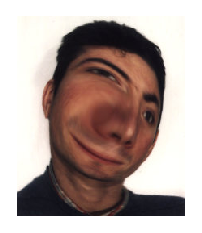
\includegraphics{img/punch_small}
后后。
}\begin{verbatim}
前前
\includegraphics{punch}
后后。
\end{verbatim}
\end{codelist}

\begin{exclamation}
    为了确保源代码的便携性、确保代码能够再不同格式下插入图像文件,有必要\emph{在指令}\dm{\backslash includegraphics}\emph{中不指定文件的扩展名}
\end{exclamation}

通常来说,我们会将\verb|\includegraphics|与环境\dm{figure}\celan{\S 2.7}结合使用。例如,图\ref{fig:5.1}依靠以下代码生成:

\begin{figure}
    \centering\includegraphics[width=5cm]{img/punch}
    \caption{罗伯特(酒后版)}
    \label{fig:5.1}
\end{figure}

\begin{dmd}
\begin{verbatim}
\begin{figure}
    \centering\includegraphics[width=5cm]{punch}
    \caption{罗伯特(酒后版)}
    \label{fig-exemple}
\end{figure}
\end{verbatim}
\end{dmd}

\begin{exclamation}
注意,环境\dm{figure}可以使图像在页面中“浮动”,而指令\verb|\includegraphics|无法做到这一点。为了防止有人漏掉这一点,再重复一遍:
\begin{center}
    \bfseries
    环境\dm{figure}可以确保\\
    图像在页面中“浮动”。\\
    这不是由指令\dm{\backslash includegraphics}\\
    来确保的。
\end{center}
\end{exclamation}

\subsection{选项}

包\textsf{graphicx}中含有若干选项,可以用于控制图像的插入过程。此处介绍其中一组最实用的选项。

\subsubsection{更改比例}

有三种调整图像尺寸的方式:

\begin{itemize}
    \item \dm{scale=}\codereplace{比例},其中\codereplace{比例}用于整体调整图片的大小,可以为正值或负值。
    \item \dm{width=}\codereplace{尺寸},可以指定图片的宽度;
    \item \dm{height=}\codereplace{尺寸},可以指定图片的高度。
\end{itemize}

\begin{codelist}[]{
    \begin{center} 
    \includegraphics[scale=0.2]{img/magma}\\
    \includegraphics[width=8.5mm]{img/magma}\\
    \includegraphics[width=2cm,
                    height=3mm]{img/magma}
    \end{center}
}\begin{verbatim}
\begin{center}
  \includegraphics[scale=0.2]{magma}\\
  \includegraphics[width=8.5mm]{magma}\\
  \includegraphics[width=2cm,
                   height=3mm]{magma}
\end{center}
\end{verbatim}
\end{codelist}

\subsubsection{旋转}

如果你希望,可以使用选项\dm{option}来让旋转图片。语法如下:

\begin{dmd}
angle=\codereplace{角}
\end{dmd}

其中\codereplace{角}以角度为单位,以逆时针方向为正方向。

\begin{codelist}[5.4]{
\includegraphics[angle=45,
                 scale=0.2]{img/magma}
}\begin{verbatim}
\includegraphics[angle=45,
                 scale=0.2]{magma}
\end{verbatim}
\end{codelist}

我们可以在文件\dm{grfguide.pdf}\jz{
  可以使用\dm{locate}或\dm{find}在你的系统中找到。
}中找到有关此扩展的详细描述,也可以参阅文档\dm{fepslatex.pdf}\jz{
  \wz{http://tug.ctan.org/tex-archive/info/epslatex/french/fepslatex.pdf}。
}。

\subsubsection{草稿模式}

选项\dm{draft}可以将图片生成为\emph{草稿}模式,即在最终文档中仅生成带有被包含文件文件名的方框。

\begin{codelist}[5.5]{
前前
\includegraphics[draft,scale=.2]{punch}
后后。
}\begin{verbatim}
前前
\includegraphics[draft,scale=.2]{punch}
后后。
\end{verbatim}
\end{codelist}

模式\dm{draft}默认在文档选项\dm{draft}指定时启用。如果想要阻止文档选项的转中效果\jz{
  例如,你希望同时看到图像和“字盒Overfull标记”。
},可以在使用指令\verb|\includegraphics|或通过\verb|\usepackage|包含扩展时使用选项\dm{final}。

\section{几个实用扩展}

接下来介绍三个可以生成带有图像文档的实用扩展。

\subsection{\textsf{subfig}}

该扩展可以管理带有若干分图的图片,分图会自动编号并能单独引用。例如:

\begin{dmd}
\begin{verbatim}
\begin{figure}[htbp]
  \begin{center}
      \leavevmode \subfloat[Magma]{%
        \label{fig-uniweria-magma}
        \includegraphics[width=2cm]{magma}}
      \hspace{2cm} \subfloat[UZMK]{%
        \label{fig-uniweria-uzmk}
        
\includegraphics[height=2cm]{uzmk}}
    \caption{Uniweria Zëkt}
    \label{fig-uniweria}
  \end{center}
\end{figure}
\end{verbatim}
\end{dmd}

\begin{figure}[htbp]
  \begin{center}
      \leavevmode \subfloat[Magma]{%
        \label{fig-uniweria-magma}
        \includegraphics[width=2cm]{img/magma}}
      \hspace{2cm} \subfloat[UZMK]{%
        \label{fig-uniweria-uzmk}
        
\includegraphics[height=2cm]{img/uzmk}}
    \caption{Uniweria Zëkt}
    \label{fig-uniweria}
  \end{center}
\end{figure}

在需要引用时,可以通过\verb|\ref{fig-uniweria}|整体引用该图,结果会展示为\ref{fig-uniweria},也可以通过对应的标签来引用分图,如使用\verb+\ref{fig-uniweria-magma}+和\verb|\ref{fig-uniweria-uzmk}|的结果分别为\ref{fig-uniweria-magma}和\ref{fig-uniweria-uzmk}。
%注意,分图没有括号。疑似这也是相关标准的来源。

\begin{ii}
有一种优雅的分图管理方法,即将每个分图打包为一个\dm{minipage}。发行版%TODO
附带的文件\dm{subfig.pdf}中说明了如何自定义环境\dm{subfigure},尤其是处理图题间的空白。
\end{ii}

\subsection{包\textsf{wrapfig}}

包\textsf{wrapfig}提供了环境\dm{wrapfigure},可以让图片在段落中浮动。此处浮动的含义不同于描述\LaTeX 的环境\dm{figure}时所用的浮动,因为此处的环境可以穿插在段落内。语法如下:

\begin{dmd}
\verb|\begin{wrapfigure}{|\codereplace{位置}\}\{\codereplace{宽度}\}\\
...\\
\verb|\end{wrapfigure}|
\end{dmd}

其中\codereplace{位置}即图片的位置(\dm{l}或\dm{r}),\codereplace{宽度}即要插入的图片宽度:

\begin{dmd}
\begin{verbatim}
\begin{wrapfigure}{r}{1.5cm}
  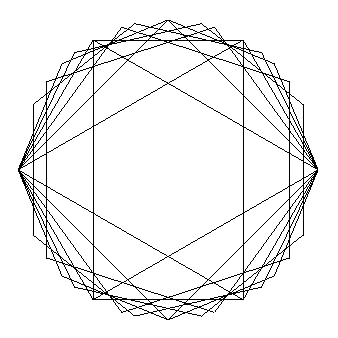
\includegraphics[width=1cm]{img/polygons}
\end{wrapfigure}

据我所知,包\textsf{wrapfig}并未
以提供\dm{dvi}文件的形式给出文档。
相反,可以在……
\end{verbatim}
\end{dmd}

\begin{wrapfigure}{r}{1.5cm}
  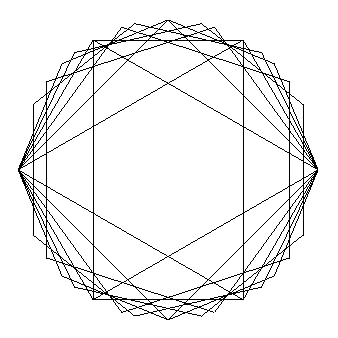
\includegraphics[width=1cm]{img/polygons}
\end{wrapfigure}

据我所知,包\textsf{wrapfig}并未以提供\dm{dvi}文件的形式给出文档。相反,可以在位于\dm{[...]/misc/wrapfig.stys}的\dm{.sty}文件自身中找到十分详细的信息。为了展示图片在段落中浮动带来的文字环绕效果,这段篇幅需要长一些,所以这里我多说一点:我们可以顺便注意到,借助一个著名的扩展——\textsf{docstrip},所有的包文档都可以“自动归纳”。这些扩展(extension),或者英文的\emph{package},包含其文档所需的代码,在安装过程中,会陆续被提取出来。\textsf{wrapfig}的作者八成没有遵循这个规则,可惜了……

\subsection{包\textsf{psfrag}}

另一个有趣的扩展是\textsf{psfrag}。它的目的是结合PostScript文件的强大和\LaTeX 方程的美观。我们想要在图片中集成数学式时,往往会遇到一个问题:大多数此类软件都不将支持数学方程作为预设。\textsf{psfrag}作者给出的解决方案中,可以使用指令\verb|\psfrag|在图中出现字符串的位置插入数学式。这样一来,使用以下方法即可生成图\ref{fig:5.3b}而非\ref{fig:5.3a}。
%此处源代码替换有问题,采用的解决方案来自https://zhidao.baidu.com/question/695901494124304244.html,即代码:
% \documentclass[border=2mm]{standalone}
% \usepackage{graphicx}
% \usepackage{psfrag}
% \begin{document}
% \psfrag{abc}{$\sin{a}$}%
% \includegraphics[width=5cm]{example.eps}
% \end{document}
% 然后执行 latex example; dvips example.dvi; epspdf example.ps
% 生成 example.pdf,在你的主文件中使用 \includegraphics{example.pdf} 导入。

\begin{figure}[ht]
  \begin{center}
      \leavevmode \subfloat[替换前]{%
        \label{fig:5.3a}
        \includegraphics[width=0.4\linewidth]{img/courbe-sans-psfrag}}
      \hspace{2cm} \subfloat[替换后]{%
        \label{fig:5.3b}
        \includegraphics[width=0.4\linewidth]{img/courbe-avec-psfrag-replace}}
    \caption{\textsf{psfrag}的使用,右图中的\LaTeX 方程替换了左图的对应部分。}%TODO 分图引用不规范
    \label{fig:5.3}
  \end{center}
\end{figure}

\begin{enumerate}
  \item 在\verb+\includegraphics{courbe}+前添加一行代码:
  
  \begin{dmd}
  \verb+\psfrag{exp(-x)*sin(10*x)}[r][r]{$e^{-x}\sin(10x)$}+
  \end{dmd}
  
  该代码可以将图例中的字符串替换为漂亮的方程。
  \item 结果在\dm{.dvi}文件中不可见。相反,\textsf{dvips}会负责使用前面的指令来修改生成的PostScript文件。
\end{enumerate}

为公式确定位置的方法即为两个参考点确定位置,其中一个参考点来自方程,另一个来自需要替换的字符串。参考点的位置由用户通过指定指令\verb|\psfrag|中间的两个可选参数确定。假设我们像这样定义了参考点:

\begin{dmd}
\backslash psfrag\{字符串\}[l][c]\{\codereplace{数学方程}\}
\end{dmd}

这样的指令对应如下对其方式:

\newlength{\tempdimdemobox}

\newcommand{\chaine}{\dm{字符串}}
\newcommand{\ekouation}{\codereplace{数学方程}}

\newcommand{\contenu}[1]{%
  \ifthenelse{\equal{#1}{b}}{\raisebox{-5pt}[0pt]}{\raisebox{5pt}[0pt]}}

\newcommand{\point}[2]{% #1 (r ou l) #2 ($\bullet$ par ex.)
  \ifthenelse{\equal{#1}{r}}{%
    \setlength{\tempdimdemobox}{\fboxsep+.5\fboxrule}}{%
    \setlength{\tempdimdemobox}{-\fboxsep-.5\fboxrule}}%
  \makebox[0pt][l]{%
    \hspace{\tempdimdemobox}\makebox[0pt]{#2}}}

\newcommand{\boxdemo}[6][-5pt]{%
  \fbox{%
    \rule[#1]{0pt}{#2}%
    \ifthenelse{\equal{#3}{r}}{% point droite
      \contenu{#5}{\footnotesize#6}%
      \point{r}{#4}}{% sinon
      \ifthenelse{\equal{#3}{l}}{% point gauche
        \point{l}{#4}%
        \contenu{#5}{\footnotesize#6}}{% sinon
        \settowidth{\tempdimdemobox}{\footnotesize#6}%
        \makebox[0pt][l]{%
          \hspace{.5\tempdimdemobox}\makebox[0pt]{#4}}%
        \contenu{#5}{\footnotesize#6}}}}}%大括号随意转行会造成空格计入方框宽度

\begin{center}
  \newlength{\zob}
  \settowidth{\zob}{\boxdemo{14pt}{c}{$\bullet$}{t}{\chaine}}
  \boxdemo{14pt}{c}{$\bullet$}{t}{\chaine}\quad 和\quad
  \boxdemo[-7pt]{18pt}{l}{$\odot$}{b}{\ekouation} \quad 叠加的结果为 \quad
  \boxdemo{14pt}{c}{$\bullet$}{t}{\chaine}\kern-.5\zob\kern-.5\fboxrule%此行对比原书有改动
  \boxdemo[-7pt]{18pt}{l}{$\odot$}{b}{\ekouation}
\end{center}

同样地,如果使用如下指令:

\begin{dmd}
  \backslash psfrag\{字符串\}[r][l]\{\codereplace{数学方程}\}
\end{dmd}

则有如下结果:

\begin{center}
  \boxdemo{14pt}{l}{$\bullet$}{t}{\chaine}\quad 和\quad
  \boxdemo[-7pt]{18pt}{r}{$\odot$}{b}{\ekouation} \quad 叠加的结果为 \quad
  \boxdemo[-7pt]{18pt}{r}{$\odot$}{b}{\ekouation}\kern-\fboxrule%
  \boxdemo{14pt}{l}{$\bullet$}{t}{\chaine}
\end{center}

在图\ref{fig:5.3b}中,我们使方程的右侧(第一个可选参数为\dm{r})与原字符串的右侧(第二个可选参数为\dm{r})对齐。该包的文档十分具有参考价值……

\begin{exclamation}
注意,如果我们使用\LaTeX 源码生成PDF文件,则只能以使用一些扭曲的操作(参见\S A%TODO
)为代价来使用包\textsf{psfrag}。
\end{exclamation}

\subsection{包\textsf{xcolor}}

扩展\textsf{xcolor}由包\textsf{graphicx}的开发团队开发,在生成彩色文本时可能会很有趣——例如,生成带有透明度的颜色。包\textsf{xcolor}可以生成以下结构:

\begin{codelist}[5.6]{
  {一些\color{red}红色}和\textcolor{cyan}{青色}的文本。

  一个\colorbox{green}{绿色}字盒。
  
  另一个\fcolorbox{blue}{yellow}{字盒}。
}\begin{verbatim}
{一些\color{red}红色}和\textcolor{cyan}{青色}的文本。

一个\colorbox{green}{绿色}字盒。

另一个\fcolorbox{blue}{yellow}{字盒}。
\end{verbatim}
\end{codelist}

在这里,我们可以理解指定颜色的方法。

\begin{itemize}
  \item 使用声明:
  
  \begin{dmd}
    \backslash color\{\codereplace{颜色}\}
  \end{dmd}

  \item 使用指令:

  \begin{dmd}
  \backslash textcolor\{\codereplace{颜色}\}\{\codereplace{文本}\}
  \end{dmd}
\end{itemize}

类似地,对于字盒,有以下方法指定颜色。

\begin{itemize}
  \item 无边框:
  
  \begin{dmd}
    \backslash colorbox\{\codereplace{填充颜色}\}\{\codereplace{内容}\}
  \end{dmd}

  \item 有边框:
  
  \begin{dmd}
    \backslash fcolorbox\{\codereplace{边框颜色}\}\{\codereplace{填充颜色}\}\{\codereplace{内容}\}
  \end{dmd}
\end{itemize}

以上两个指令生成的彩色字盒对于长度\verb|\fboxsep|比较敏感。“如果颜色没有名字\emph{怎么办}?”我听到你在\emph{嘟囔}什么了……对于这个问题,我可以马上回答:

\begin{codelist}[5.7]{
  这是
{\color[rgb]{.2,.4,.5}\bfseries 
 蓝灰色}……
}\begin{verbatim}
这是
{\color[rgb]{.2,.4,.5}\bfseries 
 蓝灰色}……
\end{verbatim}
\end{codelist}

也可以为上例中的颜色起一个“小名”:

\begin{codelist}[5.8]{
  \definecolor{bleugris}{rgb}{.2,.4,.5}
这是
{\color{bleugris}\bfseries 蓝灰色}……
}\begin{verbatim}
\definecolor{bleugris}{rgb}{.2,.4,.5}
这是
{\color{bleugris}\bfseries 蓝灰色}……
\end{verbatim}
\end{codelist}

\begin{ii}
可以注意到,除了使用“\dm{rgb}”色彩模型,也可以使用定义灰度的\dm{gray}模型。同样地,如果使用\dm{html}模型,则可以使用HTML语法来指定颜色。
\end{ii}

\begin{figure}
  \centering TODO缺图%TODO
  \caption{推荐使用的储存图像文件树状结构:图像存储在一个目录中,矢量图存储在一个目录中,EPS格式的文件存储在另外的目录中}
  \label{fig:5.4}
\end{figure}

\section{使用\textsf{make}}

\begin{exclamation}
本节面向使用部署了GNU Make(更多有关信息,请参阅相关必读资料[11])的操作系统的用户准备的。其他人可以跳过这段学习路径……
\end{exclamation}

makefile使生成过程自动化的思路有:

\begin{itemize}
  \item 使用“位图”图像文件生成EPS格式的文件;
  \item 使用带有矢量绘图软件内置格式的文件生成EPS格式的文件。
\end{itemize}

为了实现以上思路,我们需要树立一个目标,可以用以下命令行表示:

\dmh{make figs}

假设图片和图像文件分别存储在主文件所在目录下的子目录\dm{Imgs}和\dm{Figs}中,生成的EPS文件同样存储在子目录\dm{Epss}中(如图\ref{fig:5.4}所示)。此时,就可以开始定义一系列变量,来指明需要用到的不同目录:

\begin{mdframed}
\begin{verbatim}
FIGSDIR=Figs
EPSSDIR=Epss
IMGSDIR=Imgs
\end{verbatim}
\end{mdframed}

\subsection{图像转码}

首先,(作为示例)我们列出JPEG和PNG格式文件的列表,使用如下两个变量来储存列表:

\begin{mdframed}
\begin{verbatim}
PNGS=$(notdir $(wildcard $(IMGSDIR)/*.png))
JPGS=$(notdir $(wildcard $(IMGSDIR)/*.jpg))
\end{verbatim}
\end{mdframed}
  
使用函数\dm{wildcard}可以获得文件夹\verb|$(IMGSDIR)|中文件的列表,而对于每个文件,函数\dm{notdir}可以删除其“目录”的部分。最终,变量\dm{PNGS}包含:

\begin{dmd}
i.png j.png
\end{dmd}

变量\dm{JPGS}包含:

\begin{dmd}
k.jpg
\end{dmd}

接下来,我们可以从这两个变量除法,创建即将生成的EPS文件的列表(再提醒一次,EPS文件应当单独存放在一个目录中):

\begin{mdframed}
\begin{verbatim}
IMGS2EPSS=$(patsubst %,$(EPSSDIR)/%,\
          $(PNGS:.png=.eps) $(JPGS:.jpg=.eps))
\end{verbatim}
\end{mdframed}

赋值符号右侧的表达式可以将前文中两个列表中文件的扩展名改为\dm{eps},并且文件名前加上存储EPS文件的目录作为前缀。因此,\dm{IMG2EPSS}包含:

\begin{dmd}
Epss/i.eps Epss/j.eps Epss/k.eps
\end{dmd}

该列表构成了(\textsf{make}意义上)生成图像的“先决”条件。因此,按以下方式定义目标:

\begin{mdframed}
\begin{verbatim}
figs : $(IMGS2EPSS)
\end{verbatim}
\end{mdframed}

此外,也需要向\textsf{make}解释我们如何将图像文件转换为封装好的PostScript格式。可以通过如下规则描述:

\begin{mdframed}
\begin{tabbing}
\verb|abcd|\=\kill
\verb+$(EPSSDIR)/%.eps : $(IMGSDIR)/%.png+\\
$\longmapsto$\>\verb+convert $< EPS:$@ +\\
\verb+$(EPSSDIR)/%.eps : $(IMGSDIR)/%.jpg+\\
$\longmapsto$\>\verb+convert $< EPS:$@+
\end{tabbing}
\end{mdframed}

这样的规则详细描述道:我们将会用到工具\textsf{convert}\jz{
  其属于包ImageMagick,可以在\wz{http://www.imagemagick.org}获取。该工具几乎可以转换所有格式的图片。
}来将JPEG和PNG文件转换为EPS格式。

\subsubsection{转换图像文件}

图像文件的转码严格遵循同一原则。假设我们指明了一个由\textsf{xfig}生成的fig格式源文件和一个由\textsf{Inkscape}生成的svg格式源文件,则\dm{makefile}有:

\begin{mdframed}
\begin{verbatim}
FIGS=$(notdir $(wildcard $(FIGSDIR)/*.fig))
SVGS=$(notdir $(wildcard $(FIGSDIR)/*.svg))
FIGS2EPSS=$(patsubst %,$(EPSSDIR)/%,\
          $(FIGS:.fig=.eps) $(SVGS:.svg=.eps))
\end{verbatim}
\end{mdframed}

当然,两条转换规则是不同的,因为它们分别会调用\textsf{fig2dev}(\textsf{xfig}的相关工具)和\textsf{Inkscape}本身:

\begin{mdframed}
\begin{tabbing}
\verb|abcd|\=\kill
\verb+$(EPSSDIR)/%.eps : $(FIGSDIR)/%.fig+\\
$\longmapsto$\>\verb+fig2dev -L eps $< > $@+\\
\verb+$(EPSSDIR)/%.eps : $(FIGSDIR)/%.svg+\\
$\longmapsto$\>\verb+inkscape -E $@ $<+
\end{tabbing}
\end{mdframed}

最终,用于输出图像文件和图片的目标如下:

\begin{mdframed}
\begin{verbatim}
figs : $(IMGS2EPSS) $(FIGS2EPSS)
\end{verbatim}
\end{mdframed}

\section{除此之外……}

针对特殊的需求,我们可以找到大量可以生成能满足需要的图像(电路图、直方图、树形图……)的扩展。实际上,你可能在某天需要使用一个指令自动生成若干图像,这时请看看可用的不同扩展(\textsf{pstricks}、\MP……)、环境\dm{picture}及其扩展\textsf{epic}和\textsf{eepic}。加油!

\begin{ii}
目前,包TikZ的发展顺风顺水。该包可以为其优秀的用户提供使用一种依赖\LaTeX 的语言创作图画的可能。如果文档中的图以等价的形式出现多次,这种解决方案会非常有趣。该包会在本书的未来版本中介绍\yz{
  我等到花儿也谢了……
}。
\end{ii}
\chapter{科技文档}

\begin{quote}
    智慧人积存知识,愚妄人的口速致败坏。——《圣经·箴言》10:14
\end{quote}

现在,终于到了跟你聊聊所谓\emph{科技}文档特性的时刻。虽然关于数学式和其他方程的问题已经在第3章妥善解决,但还有一块骨头要啃:参考文献。对于这个问题,虽然不能一口吃个胖子,但接下来的内容可以让你大幅简化工作。在本章,我们还会解释生成索引的机制。

本章首先会介绍起草文章的几点特别之处,然后展示参考文献的生成和索引的生成,最后介绍将大篇幅文档拆解成几个小部分的实用方法。

\section{文章(article)}

为了起草一篇文章,没有什么新内容可以介绍的,我们目前为止见过的所有内容都适用。只需要注意,在文前部分中,可以使用以下指令:

\begin{itemize}
    \item \verb|\title|,定义标题;
    \item \verb|\date|,定义日期;
    \item \verb|\author|,定义作者团队;
    \item \verb|\thanks|,定义作者单位。
\end{itemize}

若要利用这些定义来插入标题,需要在\verb|\begin{document}|之\textbf{后}插入指令\verb|\maketitle|:

\begin{dmd}
\begin{verbatim}
\documentclass{article}
\title{Le seuillage à 128 : une révolution !}
\author{M. C. Orlanrien\\
        Institut du Pixel\\
        42007 Saint-Etienne---FRANCE}
\date{2 Avril 1927}
\begin{document}
\end{verbatim}
\backslash maketitle\textsl{\% 标题插到此处}\\
...\\
\verb|\end{document}|
\end{dmd}

此处重复一遍\jz{
    因为传授知识就是重复的过程。
}:标题是由指令\verb|\maketitle|生成并插入的,而不是文前部分的定义。

通常来说,会议或期刊提供的模板文件中会引入一些变化(例如使用\verb|\address|分隔作者和其地址),但基本原理是一致的。

\section{参考文献}

由两种方式可以使用\LaTeX 起草文章的参考文献部分。其中,可以称得上是“手动”的方式是,在文章中插入环境\dm{thebibliography}。另一种方式,即此处要介绍的方式,是使用\bib ,主要分为如下步骤。

\begin{enumerate}
    \item 创建一个或多个参数文件,包含\bib 格式的各条参考文献入口(entrée;文章、会议……)。这个步骤不可避免地需要我们去\emph{输入}。
    \item 在文档中,使用指令\verb|\cite|去引用这些入口。
    \item 参考文献会自动根据你选择的特殊风格排版。
\end{enumerate}

这种方法的优势是,对于每条参考文献,你只需输入一次。此外,考虑到可以使用\emph{风格文件},你不用去担心它的版式。有几十种风格文件,对应各种标准,包含期刊和其他会议所使用的标准。我们也可以在互联网上找到\bib 格式的参考文献数据库,可以在文档中直接使用。

我们重复一遍:参考文献有多种标准。但不幸的是,一些期刊偏偏喜欢指定属于自己的参考文献格式。有朝一日你在这种期刊上发表文章时,就需要去创建或调整风格文件。为了实现这一点,可以去查找工具\textsf{makebst}。

\subsection{\dm{.bib}文件}

第一个操作是构建\jz{
    \textbf{Emacs}的Auc\TeX 组件包含了很好用的\bib 模式。
}参考文献文件,其扩展名最好为\dm{.bib}。该文件需要遵循特殊的语法。首先需要知道,\bib 通过\emph{类型(type)}区分每个入口。这样一来,每个入口都带有一个文档类型:图书、文章、会议、科技报告……一共有二十多种不用的文档类型。

\begin{ii}
正常来说,我们可以在伴随\LaTeX 发行版提供的文件找到名为\bib ing的文件(命名为\dm{btxdoc.pdf}),由奥兰·帕塔什尼克(Oran Patashnik)在约二十年前创作。该文件包含有关构建\bib 格式文件方法的重要信息来源。
\end{ii}

每个入口\emph{类型}都包含一定数量描述该入口的\emph{字段(champ)}。参考文件入口的结构如下:

\begin{dmd}
@\codereplace{入口}\{\codereplace{关键描述},\\
\verb|  |\codereplace{字段$_1$}\ =\ \{...\},\\
\verb|  |\codereplace{字段$_2$}\ =\ \{...\},\\
\verb|  |...\\
\verb|  |\codereplace{字段$_n$}\ =\ \{...\},\\
\}
\end{dmd}

其中,\codereplace{入口}表示文档类型(\dm{article}、\dm{inproceedings}等),\codereplace{字段$_1$}、\codereplace{字段$_2$}……\codereplace{字段$_n$}表示参考文献入口的不同字段。这些\bib 的保留字可以以大写或小写形式输入。

符号\codereplace{关键描述}需要以唯一方法描述该文档,以备通过用于识别标签的符号\verb|\label|来重新找到。为了你能够快速上手\bib ,接下来的示例综合了三个你需要使用的基本入口。

\subsubsection{期刊文章}

有一篇期刊文章需要以如下形式输入:

\begin{dmd}
\begin{verbatim}
@article{qtz:UchArb,
author ={Uchiyama, Toshio and Arbib, Michael A.},
title = {Color Image Segmentation
         Using Competitive Learning},
journal=pami,
volume =16, number=2, pages={1197--1206},
month=dec, year=1994}
\end{verbatim}
\end{dmd}

有以下几点需要注意。

\begin{enumerate}
    \item 1
\end{enumerate}
\chapter{法文文档}

\begin{quote}
    那人说,你所赐给我,与我同居的女人,她把那树上的果子给我,我就吃了。——《圣经·创世纪》3:12
\end{quote}

了解法文文档要遵循的规则总是好的。严格说来,这些规则并不是无法逃避的准则,而更像是一些使用上的规矩。为了让文档容易可读、避免读者被打断,\emph{建议遵循}这些规则。这些使用上的建议总体上可以让文档看起来更严肃,甚至更专业。有很多关于法文排版的作品,这里给出来自国家印刷局(imprimerie nationale)的汇编材料[7],以及伊夫·佩伊卢梭(Yves Peyrousseaux)的手册[13]。

本章包含一些总结了有关\LaTeX 为实现法文变音符号而使用的字体编码方法的信息,介绍了关于排版的一些规则和用于简化法文输入过程的包\textsf{babel}。本章的末尾介绍了文档类型\dm{letter},其是为信件和传真而设计的。

\section{带有变音符号的字母的问题}

在若干年前,\TeX 的构思阶段完成的时候,其使用的字体不包含带有变音符号的字符。每个字形以7个二进制位区分,这样一共有128个字符可被编码。由于这种方法起源于美国,这128个字符中显然不包括法文中使用的带有变音符号的字符。正因如此,在很长一段时间内,那些优秀的讲法语母语的\TeX 和\LaTeX 用户不得不以一种窘迫方式去录入带有难以输入的字符的法文文档(document en \verb+fran\c{c}ais+ avec des \verb+caract{\`e}res+ assez \verb+p{\'e}nibles+ \verb+{\`a}+ taper)\yz{
    即document en français avec des caractères assez pénibles à taper。原书此处以源代码的方式展示部分单词,以展现其烦琐程度。%原书依然错误渲染了上引号和下引号
}。

今天,这些不悦不再成为人们的糟糕记忆。1990年起,一种容纳了多种语言中带变音符号的字符的字体编码被采用,称为\emph{Cork encoding}或\emph{T1编码(codage T1)}。当然,这种\TeX 编码本身和目前的字符编码标准间存在一定的联系。一些\LaTeX 包就包含了从字符编码(如iso-latin1)到字体编码(如T1编码)的“翻译”操作。

\begin{exclamation}
    于20实际90年代末出现的标准是ISO8859,带有针对称为\emph{latin1}的欧洲语言的编码方案扩展。这也是今天最常用的编码方案。然而,近年来,
\end{exclamation}
\chapter{你的回合!}

\begin{quote}
    不可与男人苟合,像与女人一样,这本是可憎恶的。

    \hfill《圣经·利未记》18:22
\end{quote}

\part{关于《关于\LaTeX 的那些你想知道却从不敢问的问题》的那些你想知道却从不敢问的问题}

\chapter*{简介}

\begin{quote}
    王女阿,你的脚在鞋中何其美好。你的大腿圆润,好像美玉,是巧匠的手做成的。你的肚脐如圆杯,不缺调和的酒。你的腰如一堆麦子,周围有百合花\jz{
        本部分的题记都取自《雅歌》,与章标题毫无关联。
    }。

    \hfill《圣经·雅歌》7:2
\end{quote}

本部分的名为“关于《关于\LaTeX 的那些你想知道却从不敢问的问题》的那些你想知道却从不敢问的问题”,旨在解释此前的各章节是如何生成的,并借此介绍已定义的用于生成你当前看到的这本书的指令和环境。本部分的目标更宏大一些,因为我们希望为有勇气的读者提供用于创建其自己的风格的坚实知识基础……

在遇到读者询问是否可以复用本文档中这样或那样的风格的问题后,我萌生了编写接下来的章节的想法。对于我来说,继续向下编写这项工作有些艰巨,因为我需要介绍的\LaTeX 知识超出了基础知识的范畴,也因此更难解释。最后,同样重要的是,在这里,我自己的巴扎中的剩货通常必须被“合理化”,才能成为可介绍的内容。这可不是件好搞的事。

在这一部分,我想介绍些生成本文档时使用的手段。我的手段不是能获得你当前看到的版式的唯一方法。例如,文档中的一些部分可以借助一些具有类似功能的包来完成,这些包甚至能比这里开发的工具生成更好的效果。

这一部分隐藏的思想是将好奇的读者领到探索\LaTeX 的小路上,并向他们展示:我们可以借助几个工具,将原指令校准到可以严格适用于他们自己的需求的程度。这些小路具有足够的普适性,可以用于按图索骥,也可以针对类似或不同的情况来调整。这里的关键,一方面是发现“\LaTeX ”内部功能的经典之处,另一方面通过创造自己的工具来获得满足感——但针对这件事,我们不宣扬“重新发明”轮子。

我尝试尽可能只介绍\LaTeX 指令。然而,有时也有必要使用一些\TeX 的功能,这里也是一个介绍这些功能的机会。因此,这一部分由三章组成。

\begin{description}
    \item[必要工具] 介绍需要了解的指令,以为接下来的工作做准备。例如,在这里,我们可以找到\LaTeX 发行版中文件结构的踪迹、切换文档弟子的思路,以及关于基于列表创建新环境的详细介绍;
    \item[装饰] 介绍了我们实现的工具,它们用于修改标题、页眉页脚、侧栏以及其他一些细枝末节的风格。
    \item[新玩具] 这里解释了本书的侧面标签、术语字典、示例、摘要、首字下沉、提示框,以及其他一些细碎的内容的创建过程。
\end{description}

\begin{qquestion}
这些章节中给出的一些解释显得有些云里雾里,即使是作者也无法理解。问题的一些解决方案是片面的。然而,对于鄙人来说,一些内容仍然很神秘。在这些情况下,段落中会插入这种“路面不平”(dos d'âne)\yz{
    原作者已经把这个标志替掉了。在源文档中可以找到名为\dm{dosdane.eps}的文件,指的就是这里说的已经被弃用的标志。
}标志。
\end{qquestion}
\chapter{必要工具}

\begin{quote}
    我所爱的,你何其美好。何其可悦,使人欢畅喜乐。你的身量好像棕树。你的两乳如同其上的果子,累累下垂。

    \hfill《圣经·雅歌》7:7
\end{quote}

在本章,我们会介绍创造比第4章中介绍的指令和环境更复杂的指令和环境所需准备的工具。此外,借着本章的介绍,我们旨在说明,此处提到的第4章需要正确消化,才能继续这一部分的阅读。本章也会介绍一些关于字体的机制,以及挖掘\LaTeX 资源的方法。

\section{赫尔克里·波洛}

\subsection{在文件中挖掘信息}

首先,为了让使用\LaTeX 写成的文档带有一些个人特色,需要知道组成你使用的\TeX 或\LaTeX 的发行版的文件的组织方法。鄙人使用了UNIX平台的发行版\TeX Live(\wz{http://www.tug.org/texlive})。在这个发行版中,我们可以在第一时间在以下目录中查阅各种包的文档:

\begin{dmd}
/usr/share/texmf-texlive/doc/latex/
\end{dmd}

这个目录中包含其他子目录,通常每个子目录对应一个包,其中就以DVI或PostScript文件的形式提供了文档。在一些情况下,需要去检查这些包的源代码。在发行版te\TeX 中,这些源代码位于:

\begin{dmd}
/usr/share/texmf-texlive/tex/latex
\end{dmd}

在同样的位置,我们通常可以为每个包找到一个目录,包含文本形式且带有扩展名\dm{sty}的源代码,在必要时也会包含相关文件。最后,为了独立于我们可以包含的包而了解\LaTeX 的默认行为,可以借助以下位置的\LaTeX 源代码:

\begin{dmd}
/usr/share/texmf-texlive/tex/latex/base/latex.ltx
\end{dmd}

对于文档类型\dm{book},还可以借助以下位置的文档类型源代码:

\begin{dmd}
/usr/share/texmf-texlive/tex/latex/base/book.cls
\end{dmd}

\subsection{检查宏}

查找指令定义的一个非常便捷的方法是在交互式会话中求助于\LaTeX 。可以直接在操作系统的命令行终端中执行以下指令:

\dmh{latex}

我的系统是这样冷冰冰地回答的:

\begin{dmd}
\begin{verbatim}
This is e-TeXk, Version 3.14159-2.1 (Web2C 7.4.5)
%&-line parsing enabled.
**
\end{verbatim}
\end{dmd}

在“赤裸裸的\TeX ”呼喊出这个冷峻的提示(\dm{**})的邀请下,我勇敢地回复了\verb|&latex|来要求加载\LaTeX 格式。没有丝毫延迟,就得到了答复:

\begin{dmd}
\begin{verbatim}
**&latex
entering extended mode
LaTeX2e <2001/06/01>
Babel <v3.7h> and hyphenation patterns for american,
french loaded.
*
\end{verbatim}
\end{dmd}

注意,提示中少了一个星号。从现在开始,我们就可以交互式地编写\LaTeX 文档了。从绝对意义商来说,这样做的乐趣不大,但从获取指令的定义和语法上来说,却很有帮助。因此,举例来说,我们可以写下这样的指令:

\begin{dmd}
\verb|*\show|\codereplace{指令}
\end{dmd}

这样可以获取\codereplace{指令}的定义。例如:

\begin{dmd}
\begin{verbatim}
*\show\mbox
> \mbox=\long macro:
\end{verbatim}
\verb|#1->\leavevmode \hbox {#1}.| \quad $\leftarrow$\textsf{此处为定义}\\
\verb+<*> \show\mbox+
\end{dmd}

其中向我们提供了指令\verb|\mbox|的定义。可以注意到,该指令被调用时,将这种调用转化为对\verb|\leavevmode|和\verb|\hbox|的调用。在好奇心的驱使下,我们继续查看指令的定义:

\begin{dmd}
\verb|*\show\hbox|\\
\verb|> \hbox=\hbox.| \quad $\leftarrow$\textsf{这是一个原语}\\
\verb|<*> \show\hbox|
\end{dmd}

可以观察到,\verb|\hbox|不是由其他指令定义而成的。在\TeX 中,这种指令称为原语(primitive)。我们的探索可以继续:

\begin{dmd}
\verb|*\show\leavevmode|\\
\verb|> \leavevmode=macro:|\\
\verb|->\unhbox \voidb@x .|\quad $\leftarrow$\backslash leavevmode\textsf{的定义}\\
\verb|<*> \show\leavevmode|
\end{dmd}

以此类推……

\section{底层工具}

\subsection{百分号图个什么?}

你可能已经注意到,有时\LaTeX 源代码中的行末带有百分号\dm{\%}。基于代码换行时文本间会自动添加空格这样的情况,百分号就有理由出现了。请看如下指令:

\begin{dmd}
\verb|\newcommand{\beurk}{bidule}|
\end{dmd}

为了增强可读性,这条指令可以拆分为多行代码:

\begin{codelist}[9.1]{
\newcommand{\beurk}{
    bidule
}
==(\beurk)==
}\begin{verbatim}
\newcommand{\beurk}{
    bidule
}
==(\beurk)==
\end{verbatim}
\end{codelist}

可以观察到,“bidule”一词的两侧出现了我们不想要的空格。为了避免这种现象,可以使用如下方式改写:


\begin{codelist}[9.2]{
\newcommand{\beurk}{%
    bidule%
}
==(\beurk)==
}\begin{verbatim}
\newcommand{\beurk}{%
    bidule%
}
==(\beurk)==
\end{verbatim}
\end{codelist}

在另一些场景下,空格会为行文带来有害的干预。定义以下环境:

\begin{dmd}
\begin{verbatim}
\newenvironment{hyperimportant}{% 
    \bfseries\itshape}{% 
    \upshape\mdseries}
\end{verbatim}
\end{dmd}

\newenvironment{hyperimportant}{% 
    \bfseries\itshape}{% 
    \upshape\mdseries}

\begin{codelist}[9.3]{
    Il est impératif
\begin{hyperimportant}
  de multiplier les sauvegardes
\end{hyperimportant}
de vos documents personnels
}\begin{verbatim}
Il est impératif
\begin{hyperimportant}
    de multiplier les sauvegardes
\end{hyperimportant}
de vos documents personnels
\end{verbatim}
\end{codelist}

如果仔细观察生成的文本,可以注意到,在粗斜体部分文本“{\bfseries\itshape de ... sauvegardes}”的两侧各有两个空格:

\begin{itemize}
    \item “{\bfseries\itshape de}”前面的两个空格分别由“\dm{impératif}”和begin条目“\verb|\begin{hyperimportant}|”后的换行引入;
    \item “{\bfseries\itshape sauvegardes}”后面的两个空格分别由“\dm{sauvegardes}”和end条目“\verb|\end{hyperimportant}|”后的换行引入。
\end{itemize}

我们可以删除换行,来证明这种观点:

\begin{codelist}[9.4]{
Il est impératif\begin{hyperimportant} de
multiplier  les
sauvegardes\end{hyperimportant} de vos
documents personnels
}\begin{verbatim}
Il est impératif\begin{hyperimportant} de
multiplier  les
sauvegardes\end{hyperimportant} de vos
documents personnels
\end{verbatim}
\end{codelist}

为了防止被这种问题牵扯精力,一般可以求助于两条用于删除双重空格的指令。对于序列之前的双重空格,可以调用指令\verb+\ignorespaces+来消除它;对于序列之后的,可以调用\verb|\unskip|。

\subsubsection{指令\dm{\backslash ignorespaces}}

该指令可以展开后续的指令,并忽略后面的所有空格:

\begin{codelist}[9.5]{
\newcommand{\truc}{ }
\newcommand{\bidule}{ }

a\truc\bidule b\par
a\ignorespaces\truc\bidule b
}\begin{verbatim}
\newcommand{\truc}{ }
\newcommand{\bidule}{ }

a\truc\bidule b\par
a\ignorespaces\truc\bidule b
\end{verbatim}
\end{codelist}

以上示例中,指令\verb|\truc|和\verb|\bidule|的唯一作用都是在被调用时生成空格。例如,以下指令会生成“\verb*|a { }b|”:

\begin{dmd}
\verb|a\truc\bidule b|
\end{dmd}

也就是说,字母a和b之间由两个空格隔开。调用指令\verb|\ignorespaces|——正如其名——可以忽略指令\verb|\truc|和\verb|\bidule|产生的空格。因此,对于前面的示例,可以使用以下指令:

\begin{dmd}
\begin{verbatim}
\newenvironment{hyperimportant}{% 
    \bfseries\itshape\ignorespaces}{\upshape\mdseries}
\end{verbatim}
\end{dmd}

这样就能删除一个空格:

\renewenvironment{hyperimportant}{% 
    \bfseries\itshape\ignorespaces}{\upshape\mdseries}

\begin{codelist}[9.6]{
    Il est impératif
\begin{hyperimportant}
    de multiplier les sauvegardes
\end{hyperimportant}
de vos documents personnels.
}\begin{verbatim}
Il est impératif
\begin{hyperimportant}
    de multiplier les sauvegardes
\end{hyperimportant}
de vos documents personnels.
\end{verbatim}
\end{codelist}

\subsubsection{指令\dm{\backslash unskip}}

如果细心一些,我们可以发现,“{\bfseries\itshape sauvegardes}”和“de”之间仍然有两个空格抵住了我们的攻击。这就到了\TeX 的原语\verb|\unskip|的用武之地:它可以删除后一个被插入的空格:

\begin{codelist}[9.7]{
    \newcommand{\truc}{ }
\newcommand{\bidule}{ }
a\truc\bidule b\par
a\truc\bidule\unskip b
}\begin{verbatim}
\newcommand{\truc}{ }
\newcommand{\bidule}{ }
a\truc\bidule b\par
a\truc\bidule\unskip b
\end{verbatim}
\end{codelist}

最后,我们环境的“正确”定义如下:

\begin{dmd}
\begin{verbatim}
\newenvironment{hyperimportant}{% 
    \bfseries\itshape\ignorespaces}{\unskip\upshape\mdseries}
\end{verbatim}
\end{dmd}

这样,就可以删除所有我们不希望插入的空格:

\renewenvironment{hyperimportant}{% 
    \bfseries\itshape\ignorespaces}{\unskip\upshape\mdseries}

\begin{codelist}[9.8]{
Il est impératif
\begin{hyperimportant}
  de multiplier les sauvegardes
\end{hyperimportant}
de vos documents personnels.
}\begin{verbatim}
Il est impératif
\begin{hyperimportant}
  de multiplier les sauvegardes
\end{hyperimportant}
de vos documents personnels.
\end{verbatim}
\end{codelist}

\subsection{字符\dm{@}}

在开始探索包的源代码时,你会发现,有很大一部分的指令名称定义中都带有字符\dm{@}。然而,在\dm{.tex}文档中,不允许执行名称带有该字符的指令。这样可以保护或限制包指令的能力范围。例如,在包\textsf{changebar}中定义了指令\verb+\cb@defpoint+,它不能被包的使用者调用。若要重定义该内部指令,需要做出以下小操作:

\begin{dmd}
\begin{verbatim}
\makeatletter
% 我们可以在这里胡说八道
\renewcommand{\@ttention}{oulala...}
\makeatother
% 但在这里就不行了
\end{verbatim}
\end{dmd}

这里举例的指令\verb+\@ttention+只有在字符\dm{@}被当作字母的情况下才能被操作。这正是\verb+\makeatletter+的作用:将字符\dm{@}转化为字母,就像其他字母一样。而指令\verb+\makeatother+可以重新赋予该字符区别于其他字母的特殊性。

\begin{exclamation}
这种操作在使用指令\verb+\usepackage+包含的风格文件中不是必需的。对于这些文件,字符\dm{@}可以当作字母使用。
\end{exclamation}

\TeX 得以更改此字符的类别的方法在10.5.1小节会详细解释。

\subsection{\TeX 的\dm{\backslash let}}

有时,修改\LaTeX 内部的指令以在其默认行为中添加功能是很有用的做法。例如,为了修改内部指令\verb+\bidule+\jz{
    好吧,这并不是一条内部指令。它只是作为愚蠢的例子而使用的指令名称……
},可以遵循以下步骤。

\begin{enumerate}
    \item 借助\TeX 的指示\verb+\let+保存该指令:
    
    \begin{dmd}
    \verb|\let\biduleORIG\bidule|
    \end{dmd}

    \item 在初始定义的基础上重新定义指令\verb+\bidule+:
    
    \begin{dmd}
    \begin{verbatim}
\renewcommand{\bidule}{%
    一些新东西\biduleORIG}
    \end{verbatim}
    \end{dmd}

    \item 如果有需要,可以借助如下指令重新回到其原定义:
    
    \begin{dmd}
    \verb+\let\bidule\biduleORIG+
    \end{dmd}
\end{enumerate}

\section{控制结构和测试}

包\textsf{ifthen}引入的结构遵循以下语法:

\begin{dmd}
\verb+\ifthenelse{+\codereplace{布尔表达式}\}\\
\{ ……若真,\LaTeX 代码……\}\\
\{ ……若假,\LaTeX 代码……\}
\end{dmd}

以及

\begin{dmd}
\verb+\whiledo{+\codereplace{布尔表达式}\}\\
\{……只要为真时,\LaTeX 代码……\}
\end{dmd}

\codereplace{布尔表达式}可以根据可以由包\textsf{ifthen}中不同指令的上下文构成,具体如下:

\begin{itemize}
    \item 表达式\codereplace{数$_1$}\dm{>}\codereplace{数$_2$}、\codereplace{数$_1$}\dm{<}\codereplace{数$_2$}及\codereplace{数$_1$}\dm{=}\codereplace{数$_2$}都可以用于比较\codereplace{数$_1$}和\codereplace{数$_2$};
    \item \verb+\equal{+\codereplace{$C_1$}\verb+}{+\codereplace{$C_2$}\dm{\}}可以根据字符串\codereplace{$C_1$}是否等于\codereplace{$C_2$}来返回真或假;
    \item \verb+\isodd{+\codereplace{数}\verb+}+在\codereplace{数}是奇数的时候返回真,否则返回假;
    \item \verb+\value{+\codereplace{计数器}\dm{\}}可以以可被布尔条件使用的形式返回\codereplace{计数器}的值;
    \item \verb+\lengthtest{\codereplace{长度检验}+\dm{\}}返回表达式\codereplace{长度检验}的结果,所谓“长度检验”包含操作符\dm{>}、\dm{<}或\dm{=}和作为运算量的\LaTeX 长度。
\end{itemize}

可以注意到,我们可以使用逻辑连接符\verb+\OR+、\verb+\AND+和\verb+\NOT+,它们在布尔表达式中扮演的正是我们所想象的角色。也可以使用操作符\verb+\(+和\verb+\)+来组合表达式。

\subsection{布尔值和相关操作符}

包\textsf{ifthen}为其朝气蓬勃的用户提供了操作布尔值的方式。可以使用指令\verb+\newboolean+声明一个布尔值:

\begin{dmd}
\verb+\newboolean{+\codereplace{布尔值标识}\}
\end{dmd}

这样就定义了一个可以以\codereplace{布尔值标识}唯一指代的布尔值。接下来,可以使用指令\verb+\setboolean+为其赋值\dm{true}或\dm{false}:

\begin{dmd}
\verb|\setboolean{|\codereplace{布尔值标识}\}\{\codereplace{值}\}
\end{dmd}

当然,可以在控制结构\celan{\S 9.3}中使用以此种方式创建的布尔值,例如:

\begin{dmd}
\verb|\ifthenelse{\boolean{|\codereplace{布尔值标识}\}\}\\
\{……\codereplace{布尔值标识}为真时的\LaTeX 代码……\}\\
\{……\codereplace{布尔值标识}为假时的\LaTeX 代码……\}
\end{dmd}

这里提议了解一下前面内容中的\TeX 版本。实际上,我们可以在\LaTeX 包中找到使用\TeX 编写的代码,特别是对结构“若--则--否则”的使用。如下示例使用了\TeX 定义了新的布尔值\yz{
    其中,imprimante couleur意为“彩色打印机”。
}:

\begin{dmd}
\verb|\newif\ifimprimantecouleur|
\end{dmd}

使用如下指令将其置为假:

\begin{dmd}
\verb|\imprimantecouleurfalse|
\end{dmd}

使用如下指令将其置为真:

\begin{dmd}
\verb|\imprimantecouleurtrue|
\end{dmd}

接下来,就可以在\TeX 模式的结构“若--则--否则”中操作这个布尔值:

\begin{dmd}
\backslash ifimprimantecouleur\\
... \textsl{\% 针对彩色打印机的代码}\\
\backslash else\\
... \textsl{\% 针对黑白打印机的代码}
\end{dmd}

\subsection{示例}

我们希望通过编写指令来生成阶乘函数的展开\jz{
    有人整天没什么事情可做……
},使得以下方法可以生成预期效果:

\begin{codelist}[9.9]{
    9的阶乘可以表达为:
    \begin{displaymath}
        9!=9\times 8\times 7\times 6\times 5\times 4\times 3\times 2\times 1
    \end{displaymath}
}\begin{verbatim}
9的阶乘可以表达为:
\begin{displaymath}
    9!=\itfactorielle{9}
\end{displaymath}
\end{verbatim}
\end{codelist}

解决该问题的一种方法是,编写一个指令,其中包含循环\verb|\whiledo|:

\begin{dmd}
    \begin{verbatim}
\verb|\newcommand{\itfactorielle}[1]{%
    \setcounter{cptfact}{#1} % 使用一个计数器来存储变量
    \whiledo{\value{cptfact}>1}{ % 只要变量大于1
    \thecptfact\times % 显示一个乘号
    \addtocounter{cptfact}{-1}} % 计数器递减
1} % 在末尾显示1
    \end{verbatim}
\end{dmd}

当然,需要声明计数器:

\begin{dmd}
\verb+\newcounter{cptfact}+
\end{dmd}

可以注意到,在“只要……”循环中的布尔条件中,我们调用了指令\verb|\value|来比较计数器的值和1。更迂回的办法是,我们可以以递归的方式来实现这个指令:

\begin{dmd}
\begin{verbatim}
\newcommand{\recfactorielle}[1]{ % 递归的方式
\setcounter{cptfact}{#1} % 为计数器赋值
\ifthenelse{#1>1}{ % 如果值大于1
    \thecptfact\times % 显示计数器,并紧跟一个乘号
    \addtocounter{cptfact}{-1} % 计数器递减
    \recfactorielle{\thecptfact}} % 做一次递归调用
{1}} % 否则(即值为1)显示1
\end{verbatim}
\end{dmd}

该指令当然与之前的方法生成相同的结果。注意到,在\verb|\ifthenelse|的条件中,我们将一个数(\dm{\#1})与另一个数(1)作比较。我们也能注意到,\verb|\times|的出现说明了该指令需要在数学模式中执行。如果有需要,我们也可以通过指令\verb|\ensuremath|\celan{\S 4.5.1}来避开这个问题。

在你当前阅读的这个文档中,使用了\verb|\whiledo|\verb|\ifthenelse|来生成表\ref{tab:C.22},以及第7章中的表??\yz{
    原文此处链接丢失。
}。首先,我们创建了用于以如下形式显示一个符号的指令:

\newcommand{\affsymb}[2]{%
\framebox{% un cadre
\parbox[][16pt][b]{1em}{% autour d'une boîte paragraphe 
\centering% de 16 pt de hauteur, 1em de large,
\Pisymbol{#1}{#2}\\% dont le contenu centré 
\tiny#2}}}

\begin{codelist}[9.10]{
    \affsymb{pzd}{249} \affsymb{pzd}{75}
    \affsymb{pzd}{221} \affsymb{pzd}{88}
}\begin{verbatim}
\affsymb{pzd}{249} \affsymb{pzd}{75}
\affsymb{pzd}{221} \affsymb{pzd}{88}
\end{verbatim}
\end{codelist}

这个指令如下:

\begin{dmd}
\begin{verbatim}
\newcommand{\affsymb}[2]{% 
    \framebox{% un cadre
        \parbox[][16pt][b]{1em}{ % 使用段落字盒框起
            \centering % 字盒高度为16pt,宽度为1em
            \Pisymbol{#1}{#2}\\ % 字盒的内容居中 
            \tiny#2}}} % 字盒的内容由符号和其编号组成
\end{verbatim}
\end{dmd}

参数\dm{\#1}是字体名(\dm{pzd}或\dm{psy}),参数\dm{\#2}是符号\celan{\S C}的编号。如果你一路阅读本书到这里,并且已经仔细阅读了第4章,尤其是4.4节,那么这段指令对你来说没什么特别的……接下来,我们定义一个指令,用于显示一系列符号:

\newcounter{clig}
\newcounter{csym}
\newcounter{cligmax}
\newcounter{ccol}
\newcounter{ccolmax}

\newcommand{\symboles}[4][0]{%
\setcounter{clig}{0}% Mise à zéro des compteurs de ligne 
\setcounter{ccol}{0}% et de colonne 
\setcounter{cligmax}{#3}% arguments 3 et 4 pour fixer 
\setcounter{ccolmax}{#4}% le nbre max de colonnes et de lignes 
% Pour chaque ligne : 
\whiledo{\value{clig}<\value{cligmax}}{%
\setcounter{ccol}{0}% remise à zéro du compteur de colonne 
% et pour chaque colonne : 
\whiledo{\value{ccol}<\value{ccolmax}}{%
% on calcule le numéro du symbole 
\setcounter{csym}{%
         \value{clig}*\value{ccolmax}+\value{ccol}+#1}
% si sa valeur est inférieure à 256 
\ifthenelse{\value{csym}<256}{%
\affsymb{#2}{\thecsym}}{% on l'affiche
\mbox{}}% sinon on créé un boîte vide 
\stepcounter{ccol}}% on passe à la colonne suivante
\stepcounter{clig}% on passe à la ligne suivante
% on saute une ligne, sauf à la fin 
\ifthenelse{\value{clig}<\value{cligmax}}{\\}{}}}

\begin{codelist}[9.11]{
如下是Zapf Dingbats字体下的一些符号,
从40号开始,排列成3行6列:
\begin{center}
    \symboles[40]{pzd}{3}{6}
\end{center}
}\begin{verbatim}
如下是Zapf Dingbats字体下的一些符号,
从40号开始,排列成3行6列:
\begin{center}
    \symboles[40]{pzd}{3}{6}
\end{center}
\end{verbatim}
\end{codelist}

如下所示,是指令\verb|\symboles|:

\begin{dmd}
\begin{verbatim}
\newcommand{\symboles}[4][0]{%
    \setcounter{clig}{0} % 行计数器置0
    \setcounter{ccol}{0} % 列计数器置0
    \setcounter{cligmax}{#3} % 变量3和4分别用于控制
    \setcounter{ccolmax}{#4} % 行数和列数的最大值
    % 对于每行:
    \whiledo{\value{clig}<\value{cligmax}}{%
        \setcounter{ccol}{0} % 将列计数器重新置0
        % 对于某列: 
        \whiledo{\value{ccol}<\value{ccolmax}}{%
            % 计算符号的编号
            \setcounter{csym}{%
                \value{clig}*\value{ccolmax}+\value{ccol}+#1}
            % 若值小于256 
            \ifthenelse{\value{csym}<256}{%
                \affsymb{#2}{\thecsym}}{ % 显示该符号
                \mbox{}}% 否则,创建空字盒
            \stepcounter{ccol}} % 进到下一列
        \stepcounter{clig} % 进到下一行
    % 换行,除非到达结尾
    \ifthenelse{\value{clig}<\value{cligmax}}{\\}{}}}
\end{verbatim}
\end{dmd}

当然,需要使用指令\verb|\newcounter|声明其中的五个计数器。

\begin{codelist}[9.12]{
    我知道,你尤其好奇在计数器到达边界时,
    指令会怎样处理:
\begin{center}
    \symboles[240]{psy}{3}{6}
\end{center}
}\begin{verbatim}
我知道,你尤其好奇在计数器到达边界时,
指令会怎样处理:
\begin{center}
    \symboles[240]{psy}{3}{6}
\end{center}
\end{verbatim}
\end{codelist}

\subsection{判断页码的奇偶性}

有个十分日常的实践,就是创建可以根据页码的奇偶性显示不同内容的指令。我们接下来就来研究下这个事情。在英文问答网站[1]的“Finding if you're on an odd or an even page”入口可以找到,以下天真做法不能得到预期效果:

\begin{dmd}
\begin{verbatim}
\ifthenelse{\isodd{\value{page}}} 
{……对于奇数页……}
{……对于偶数页……}
\end{verbatim}
\end{dmd}

这是因为,在\emph{两个页面的交界处}检测时,页码计数器可能不会被更新:如果在页面开头请求的页码计数器,它会返回前一页的页码……这要归咎于\TeX 实现换页时的处理方法。为了避开这个问题,有很多可用的解决方案。此处采用的方法是使用包\textbf{chngpage}。它使得我们可以在想要检测页码奇偶性的时候人工插入一个\verb|\label|。

所以,在页码奇偶性的检测过程被评估成位于两页的交接处时,可以这样写:

\begin{dmd}
\begin{verbatim}
\checkoddpage% \ifcpoddpage
    ……对于奇数页……
\else
    ……对于偶数页……
\fi 
\end{verbatim}
\end{dmd}

\section{字体}

\subsection{“三个”字体族的游戏}

为了保持\LaTeX 文档中字体外形的一致性,三个字体族被定义:

\begin{enumerate}
    \item 罗马族,正如此处所展现的;
    \item \textsf{非衬线族,正如此处所展现的;}
    \item \dm{打字机族,对于使用英文的人,也称\emph{typewriter}族——你无疑没办法避开这个字体族,因为你正在阅读的这行文字正属于打字机族。}
\end{enumerate}

需要注意,默认的这三个字体族由其作者(克努特本人)赐名“计算机现代体”(英:Computer Modern),设计的目的是可以在同一文档内呈现得和谐。基于这样的想法,需要始终注意使这三个字体族在视觉上“相容”。\LaTeX 的各发行版通常提供了一些用以在文档中使用PostScript字体的包,其中就有著名\jz{
    但过时。现在推荐使用包\textsf{mathptmx}。
}的包\textsf{times}:

\begin{enumerate}
    \item {\fontencoding{T1} \fontfamily{ptm} \selectfont 对于罗马族,使用Times,正如此处所展现的;} 
    \item {\fontencoding{T1} \fontfamily{phv} \selectfont 对于非衬线族,使用Helvetica,正如此处所展现的;}
    \item {\fontencoding{T1} \fontfamily{pcr} \selectfont 对于打字机族,使用Courier。}
\end{enumerate}

另外,还有包\textsf{newcent}:

\begin{itemize}
    \item {\fontencoding{T1} \fontfamily{pnc} \selectfont 对于罗马族,使用New Century,正如此处所展现的;} 
    \item {\fontencoding{T1} \fontfamily{pag} \selectfont 对于非衬线族,使用Avant Garde,正如此处所展现的;}
    \item {\fontencoding{T1} \fontfamily{pcr} \selectfont 对于打字机族,使用Courier。}
\end{itemize}

\subsection{字体的指定和字体属性}

\LaTeX 中,字符的字体(fonte\jz{
    fonte这个术语参考了印刷铅字……
}或police)由多个特性定义,这正是2.1节提到的问题。为了借助接下来会出现的指令来指定字体,需要进行如下约定:

\begin{itemize}
    \item 除少数特殊情况外,我们使用T1编码;
    \item 使用一组字符序列来区分字体族,如\dm{cmr}代表\emph{计算机现代体罗马族(Computer Modern roman)}、\dm{ptm}代表\emph{PostScript Times体},等等;
    \item 使用一组字符序列来表示字重,如\dm{m}代表“中等”、\dm{b}代表加粗、\dm{bx}代表“加粗伸展”(gras étendu,英:bold extended;即字母加粗且更宽),等等;
    \item 使用一组字符序列来表示字体样式(allure,\emph{英:shape}),如\dm{n}d代表“常规”、\dm{it}代表“意大利”、\dm{sl}代表“倾斜”(英:slanted),等等。
\end{itemize}

\subsubsection{“计算机现代”字体系列}

这一套字体由唐纳德·克努特绘制,由\LaTeX 默认使用。使用指令\verb|\emph|、\verb|\textbf|等时,会自动选用其中的字体。

\newlength{\extrarowheight}

\newenvironment{decritfonte}[3][T1]{%
  \begin{center}
    \setlength{\extrarowheight}{2pt}
    \begin{tabular}{|l|c|c|c|}\hline%
      \multicolumn{1}{|c|}{#2#3)}&
      \multicolumn{3}{c|}{编码方式:#1}\\
      \hline
    }%
    {\end{tabular}
  \end{center}
}

\newcommand{\testefonte}[4]{%
    \fontencoding{#1}%
    \fontfamily{#2}%
    \fontseries{#3}%
    \fontshape{#4}%
    \selectfont}

\newcommand{\phrasetest}{machin Bidule Chouette chose}

\newcommand{\descriptionfonte}[5][T1]{%
  {\testefonte{#1}{#2}{#3}{#4}\phrasetest}&#3&#4&#5\\
  \hline}

  \begin{decritfonte}{计算机现代体罗马族(Computer Modern roman,}{cmr}
    \descriptionfonte{cmr}{m}{n}{常规}
    \descriptionfonte{cmr}{m}{it}{意大利}
    \descriptionfonte{cmr}{m}{sl}{倾斜}
    \descriptionfonte{cmr}{m}{sc}{小型大写}
    \descriptionfonte{cmr}{bx}{n}{加粗伸展常规}
    \descriptionfonte{cmr}{bx}{it}{加粗伸展意大利}
    \descriptionfonte{cmr}{bx}{sl}{加粗伸展倾斜}
    \descriptionfonte{cmr}{b}{n}{加粗常规}
  \end{decritfonte}
  
  \begin{decritfonte}{计算机现代体非衬线族(Computer Modern sans sérif,}{cmss}
    \descriptionfonte{cmss}{m}{n}{常规}
    \descriptionfonte{cmss}{m}{sl}{倾斜}
    \descriptionfonte{cmss}{bx}{n}{加粗伸展常规}
    \descriptionfonte{cmss}{sbc}{n}{半加粗紧缩常规}
  \end{decritfonte}
  
  \begin{decritfonte}{计算机现代体打字机族(Computer Modern typewriter,}{cmtt}
    \descriptionfonte{cmtt}{m}{n}{常规}
    \descriptionfonte{cmtt}{m}{it}{意大利}
    \descriptionfonte{cmtt}{m}{sl}{倾斜}
    \descriptionfonte{cmtt}{m}{sc}{小型大写}
  \end{decritfonte}
  
  \begin{decritfonte}{计算机现代体斐波那契族(Computer Modern fibonacci,}{cmfib}
    \descriptionfonte{cmfib}{m}{n}{常规}
  \end{decritfonte}
  
  \begin{decritfonte}{计算机现代体滑稽罗马族(Computer Modern funny roman,}{cmfr}
    \descriptionfonte{cmfr}{m}{n}{常规}
    \descriptionfonte{cmfr}{m}{it}{意大利}
  \end{decritfonte}
  
  \begin{decritfonte}{计算机现代体登喜路族(Computer Modern dunhil,}{cmdh}
    \descriptionfonte{cmdh}{m}{n}{常规}
  \end{decritfonte}

\subsubsection{混凝土体}

{\fontencoding{T1}\fontfamily{ccr}\fontseries{m}\fontshape{n}\selectfont 混凝土体(fontes en béton)是由克努特为其名为《实用数学》( \emph{Mathématiques concrètes},英:\emph{Concrete Mathematics}})的图书而绘制的\yz{
    英文的concrete一词既有“混凝土”的含义,又有“实用”的含义。
}。使用包\textsf{beton}可以在文档中切换该字体。

\begin{decritfonte}[T1]{混凝土体(Concrete fonts,}{ccr}
    \descriptionfonte{ccr}{m}{n}{常规}
    \descriptionfonte{ccr}{m}{sc}{小型大写}
    \descriptionfonte{ccr}{m}{sl}{倾斜}
    \descriptionfonte{ccr}{m}{it}{意大利}
\end{decritfonte}

\subsubsection{“哥特风格”字体}

{\fontencoding{U}\fontfamily{yswab}\fontseries{m}\fontshape{n}\selectfont 下面的这些字体属于哥特风格字体族(famille gothique),只有在使用目的特别明确的情况下才能使用,否则文字会极难阅读——正如这里所展示的一样。此外,你可能已经放弃读下去了,所以我可以说点脏话:yi tuo dabian……\\
}

\begin{decritfonte}[U]{哥特体(Gothique,}{ygoth}
\descriptionfonte[U]{ygoth}{m}{n}{---}
\end{decritfonte}
\begin{decritfonte}[U]{德文尖角体(Fraktur,}{yfrak}
\descriptionfonte[U]{yfrak}{m}{n}{---}
\end{decritfonte}
\begin{decritfonte}[U]{施瓦巴赫体(Schwabacher,}{yswab}
\descriptionfonte[U]{yswab}{m}{n}{---}
\end{decritfonte}

\subsubsection{PostScript字体}

下面展示的字体通常可以免费获取,而且在大多数情况下打印机都预装了这些字体。

\begin{decritfonte}{Times(}{ptm}
    \descriptionfonte{ptm}{m}{n}{常规}
    \descriptionfonte{ptm}{m}{it}{意大利}
    \descriptionfonte{ptm}{m}{sl}{倾斜}
    \descriptionfonte{ptm}{m}{sc}{小型大写}
    \descriptionfonte{ptm}{b}{n}{加粗}
  \end{decritfonte}
  
  \begin{decritfonte}{Palatino(}{ppl}
    \descriptionfonte{ppl}{m}{n}{常规}
    \descriptionfonte{ppl}{m}{it}{意大利}
    \descriptionfonte{ppl}{m}{sl}{倾斜}
    \descriptionfonte{ppl}{m}{sc}{小型大写}
    \descriptionfonte{ppl}{b}{n}{加粗}
  \end{decritfonte}
  
  \begin{decritfonte}{Charter(}{bch}
    \descriptionfonte{bch}{m}{n}{常规}
    \descriptionfonte{bch}{m}{it}{意大利}
    \descriptionfonte{bch}{m}{sl}{倾斜}
    \descriptionfonte{bch}{m}{sc}{小型大写}
    \descriptionfonte{bch}{b}{n}{加粗}
  \end{decritfonte}
  
  \begin{decritfonte}{New Century(}{pnc}
    \descriptionfonte{pnc}{m}{n}{常规}
    \descriptionfonte{pnc}{m}{it}{意大利}
    \descriptionfonte{pnc}{m}{sl}{倾斜}
    \descriptionfonte{pnc}{m}{sc}{小型大写}
    \descriptionfonte{pnc}{b}{n}{加粗} 
  \end{decritfonte}
  
  \begin{decritfonte}{Bookman(}{pbk}
    \descriptionfonte{pbk}{m}{n}{常规}
    \descriptionfonte{pbk}{m}{it}{意大利}
    \descriptionfonte{pbk}{m}{sl}{倾斜}
    \descriptionfonte{pbk}{m}{sc}{小型大写}
    \descriptionfonte{pbk}{b}{n}{加粗}
  \end{decritfonte}

  \begin{decritfonte}{Helvetica(}{phv}
    \descriptionfonte{phv}{m}{n}{常规} 
    \descriptionfonte{phv}{m}{sl}{倾斜}
    \descriptionfonte{phv}{m}{sc}{小型大写}
    \descriptionfonte{phv}{b}{n}{加粗}
    \descriptionfonte{phv}{bc}{n}{加粗紧缩}
  \end{decritfonte}
  
  \begin{decritfonte}{Avant Garde(}{pag}
    \descriptionfonte{pag}{m}{n}{常规}
    \descriptionfonte{pag}{m}{sl}{倾斜}
    \descriptionfonte{pag}{m}{sc}{小型大写}
    \descriptionfonte{pag}{b}{n}{加粗}
  \end{decritfonte}
  
  \begin{decritfonte}{Courier(}{pcr}
    \descriptionfonte{pcr}{m}{n}{常规}
    \descriptionfonte{pcr}{m}{sl}{倾斜}
    \descriptionfonte{pcr}{m}{sc}{小型大写}
    \descriptionfonte{pcr}{b}{n}{加粗}
  \end{decritfonte}
  
  \begin{decritfonte}{Zapf Chancery(}{pzc}
    \descriptionfonte{pzc}{m}{n}{常规}
  \end{decritfonte}

  \subsection{切换字体}

  \subsubsection{全局切换字体}

  我们多少可以使用\LaTeX 发行版中的标准包来切换字体:

  \begin{description}
    \item[\textsf{mathptmx}] 用于“丑陋”的Times New Roman;
    \item[\textsf{newcent}] 用于New Century;
    \item[\textsf{mathpazo}] 用于Palatino;
    \item[……] 一些只在你使用的发行版中的包……
  \end{description}

  如果我们去查看文件\dm{newcent.sty}的内容,可以轻松地发现以下指令:

  \begin{dmd}
  \begin{verbatim}
\renewcommand{\rmdefault}{pnc}
\renewcommand{\sfdefault}{pag}
\renewcommand{\ttdefault}{pcr}
  \end{verbatim}
  \end{dmd}

正如9.4.1小节所说,这代表着,通过为三个字体族——“罗马”、“非衬线”,以及“打字机”指定\LaTeX 的标准名,我们重新定义了它们。如\dm{pcn}代表PostScript NewCentury、\dm{pag}代表PostScript AvantGarde等。这些标准名在9.4.2小节的表格中已经给出。

\subsubsection{局部切换字体}

在行文中,可以以以突出必要段落的方式来局部切换字体:

\begin{codelist}[9.13]{
    {\fontencoding{T1} \fontfamily{cmfr}\selectfont  On passe
    en ``Funny Roman'' et même qu'on peut
    faire de l'\emph{italique}... c'est
    dingue !} Et hop nous voila de nouveau
    en \dm{\backslash rmdefault}
}\begin{verbatim}
{\fontfamily{cmfr}\selectfont  On passe
  en ``Funny Roman'' et même qu'on peut
  faire de l'\emph{italique}... c'est
  dingue !} Et hop nous voila de nouveau
  en \verb+\rmdefault+
\end{verbatim}
\end{codelist}

在\verb|\selectfont|前可以使用调用的指令如下:

\begin{itemize}
    \item \verb|\fontencoding|指定编码方式;
    \item \verb|\fontfamily|像使用参数一样指定字体族(\dm{cmr}代表Computer Modern、\dm{ptm}代表PostScript Times等);
    \item \verb|\fontseries|指定字重(\dm{b}标识加粗、\dm{m}代表中等字重等);
    \item \verb|\fontshape|指定样式(\dm{n}表示常规、\dm{sl}表示倾斜等);
    \item \verb|\fontsize|带有两个参数,可以指定字号和相邻两行间的距离。
\end{itemize}

请看以下示例:

\begin{codelist}[9.14]{
    {\fontencoding{T1} \fontfamily{ppl}\fontseries{b}%
  \fontsize{1.8cm}{2cm}\selectfont
  Big!}
  
Et nous voila de nouveau en
\dm{\backslash rmdefault}
}\begin{verbatim}
{\fontfamily{ppl}\fontseries{b}%
  \fontsize{1.8cm}{2cm}\selectfont
  Big!}

Et nous voila de nouveau en
\verb+\rmdefault+
\end{verbatim}
\end{codelist}

最后,如果我们调用指令时,总是重复使用各种属性都完全相同的字体,则可以借助指令\verb|\DeclareFixedFont|。该指令可以接受六个参数(名称、编码方式、族、自重、风格、字号),以便我们像使用指令一样去在接下来的文本中使用:

\begin{codelist}[9.15]{
\DeclareFixedFont{\toupiti}
{T1}{pag}{m}{n}{3pt}
Avant {\toupiti bon bé là à moins d'avoir
une bonne loupe vous ne serez pas capable
de lire ce texte} après.
}\begin{verbatim}
\DeclareFixedFont{\toupiti}
{T1}{pag}{m}{n}{3pt}
Avant {\toupiti bon bé là à moins d'avoir
une bonne loupe vous ne serez pas capable
de lire ce texte} après.
\end{verbatim}
\end{codelist}


% \begin{appendices}
%     \section{附录}
% \end{appendices}
\end{document}